%Crosswords_lexVg-solve.tex	aim-50-pos-solve.tex		langford2-solve.tex		randsJC2500-solve.tex
%a5-solve.tex			kakuroext_easy-solve.tex	langford4-solve.tex		randsJC5000-solve.tex

\clearpage

\begin{figure}
  \begin{minipage}[b][10cm][s]{0.45\textwidth}
    \centering
    \vfill
    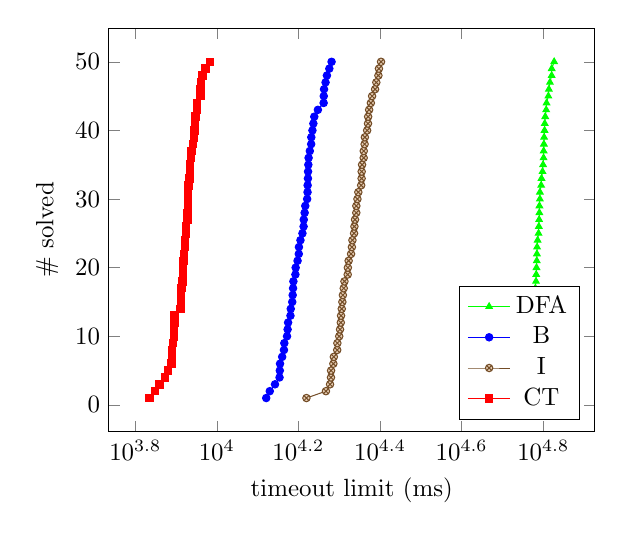
\begin{tikzpicture}[scale=0.9]
      \begin{axis}[
    xmode=log,
    every axis plot/.style={thin},
    xlabel={timeout limit (ms)},
    ylabel={\# solved},
    legend pos=south east
    % table/create on use/cumulative distribution/.style={
    %   create col/expr={\pgfmathaccuma + \thisrow{f(x)}}   
    % }
    ]
    \addplot 
    [mark=triangle*,
    mark size=1.5,
    mark options={solid},
    green] 
    coordinates {
    (51125.785, 1)
(54263.257, 2)
(56487.527, 3)
(56702.786, 4)
(56985.792, 5)
(57276.885, 6)
(57622.584, 7)
(58132.270, 8)
(58140.300, 9)
(58355.175, 10)
(58676.203, 11)
(59158.883, 12)
(59632.816, 13)
(59713.900, 14)
(59728.215, 15)
(60269.934, 16)
(60313.648, 17)
(60549.505, 18)
(60622.637, 19)
(60711.449, 20)
(60810.980, 21)
(60862.784, 22)
(60914.293, 23)
(61100.454, 24)
(61428.994, 25)
(61523.477, 26)
(61625.366, 27)
(61712.915, 28)
(61729.236, 29)
(61886.596, 30)
(61900.845, 31)
(62341.893, 32)
(62455.546, 33)
(62817.572, 34)
(63010.646, 35)
(63184.232, 36)
(63221.376, 37)
(63304.994, 38)
(63379.424, 39)
(63540.272, 40)
(63613.419, 41)
(63781.589, 42)
(64128.455, 43)
(64263.902, 44)
(64924.220, 45)
(65113.900, 46)
(65508.695, 47)
(66133.866, 48)
(66157.482, 49)
(67076.860, 50)
    };

    \addplot 
    [blue,
    mark=*,
    mark size=1.5,
    mark options={solid}]
    coordinates {
    (13210.645, 1)
(13478.699, 2)
(13880.904, 3)
(14240.906, 4)
(14262.586, 5)
(14281.012, 6)
(14453.879, 7)
(14601.257, 8)
(14630.915, 9)
(14856.229, 10)
(14906.587, 11)
(14947.426, 12)
(15147.432, 13)
(15173.599, 14)
(15300.351, 15)
(15338.350, 16)
(15370.471, 17)
(15400.162, 18)
(15575.398, 19)
(15599.555, 20)
(15767.367, 21)
(15876.487, 22)
(15890.540, 23)
(16026.936, 24)
(16207.081, 25)
(16313.213, 26)
(16328.178, 27)
(16410.911, 28)
(16468.425, 29)
(16641.910, 30)
(16678.794, 31)
(16689.212, 32)
(16716.749, 33)
(16728.322, 34)
(16755.929, 35)
(16780.814, 36)
(16896.779, 37)
(17026.619, 38)
(17037.921, 39)
(17147.387, 40)
(17237.324, 41)
(17326.549, 42)
(17685.575, 43)
(18266.956, 44)
(18281.157, 45)
(18310.293, 46)
(18466.165, 47)
(18608.783, 48)
(18864.433, 49)
(19102.683, 50)
    };

    \addplot [brown!60!black,
    mark options={fill=brown!40},
    mark=otimes*,
    mark size=1.5]
    coordinates {
    (16575.843, 1)
(18505.000, 2)
(18940.008, 3)
(19038.980, 4)
(19049.304, 5)
(19298.221, 6)
(19348.596, 7)
(19719.698, 8)
(19737.753, 9)
(19947.661, 10)
(20036.932, 11)
(20122.714, 12)
(20152.397, 13)
(20232.116, 14)
(20302.198, 15)
(20360.843, 16)
(20458.853, 17)
(20543.247, 18)
(20924.864, 19)
(20941.580, 20)
(21033.055, 21)
(21323.434, 22)
(21424.912, 23)
(21488.205, 24)
(21690.524, 25)
(21732.563, 26)
(21805.424, 27)
(21961.943, 28)
(21968.175, 29)
(22103.640, 30)
(22217.515, 31)
(22576.655, 32)
(22629.332, 33)
(22640.426, 34)
(22690.290, 35)
(22898.044, 36)
(22906.588, 37)
(23018.632, 38)
(23049.661, 39)
(23346.986, 40)
(23464.371, 41)
(23482.242, 42)
(23611.320, 43)
(23844.593, 44)
(24011.531, 45)
(24420.146, 46)
(24590.635, 47)
(24882.878, 48)
(24954.062, 49)
(25252.813, 50)
    };

    \addplot 
    [red,
    mark size=1.5,
    mark=square*]
    coordinates {
    (6834.272, 1)
(7049.566, 2)
(7238.120, 3)
(7457.754, 4)
(7598.772, 5)
(7739.737, 6)
(7771.586, 7)
(7772.970, 8)
(7812.433, 9)
(7861.439, 10)
(7862.003, 11)
(7867.552, 12)
(7871.233, 13)
(8146.006, 14)
(8162.853, 15)
(8169.022, 16)
(8197.217, 17)
(8246.900, 18)
(8258.157, 19)
(8262.374, 20)
(8291.516, 21)
(8318.251, 22)
(8342.451, 23)
(8355.561, 24)
(8389.425, 25)
(8401.690, 26)
(8470.665, 27)
(8475.034, 28)
(8489.871, 29)
(8495.761, 30)
(8507.506, 31)
(8510.152, 32)
(8560.945, 33)
(8587.622, 34)
(8588.072, 35)
(8642.789, 36)
(8662.209, 37)
(8738.285, 38)
(8798.802, 39)
(8820.422, 40)
(8831.432, 41)
(8851.771, 42)
(8928.438, 43)
(8949.293, 44)
(9107.856, 45)
(9118.812, 46)
(9135.516, 47)
(9225.896, 48)
(9370.806, 49)
(9607.234, 50)
    };
    \legend{DFA,B,I,CT}
  \end{axis}

    \end{tikzpicture}
    \vfill
    \caption{\textbf{A5}.}
    \vspace{\baselineskip}
  \end{minipage}\qquad
  \begin{minipage}[b][10cm][s]{0.45\textwidth}
    \centering
    \vfill
    \begin{tikzpicture}[scale=0.9]
      \begin{axis}[
    xmode=log,
    every axis plot/.style={thin},
    xlabel={timeout limit (ms)},
    ylabel={\% solved},
    legend pos=south east,
    cycle list/Set1-6,
            % define fill color for the marker
            mark list fill={.!75!white},
            mark options={solid},
            cycle multiindex* list={
                Set1-6
                    \nextlist
                [3 of]linestyles
                    \nextlist
                very thick
                \nextlist
                mark=o,
                mark=*,
                mark=square,
                mark=triangle,
                mark=+
            },
    ]

    \addplot
    coordinates {
      (1609830, 50)
      
    };
    \addplot
    coordinates {
      (302190, 50)
      (482210, 100)
      
    };
    \addplot
    coordinates {
      (396530, 50)
      (608250, 100)
      
    };
    \addplot
    coordinates {
      (32160, 50)
      (37170, 100)
      
    };
    

    \legend{ DFA, B, I, \textbf{CT} }
  \end{axis}

    \end{tikzpicture}
    \vfill
    \caption{\textbf{A10}.}
    \vspace{\baselineskip}
  \end{minipage}\qquad
\end{figure}

\begin{figure}
  \begin{minipage}[b][10cm][s]{0.45\textwidth}
    \centering
    \vfill
    \begin{tikzpicture}[scale=0.9]
      \begin{axis}[
    xmode=log,
    every axis plot/.style={thin},
    xlabel={timeout limit (ms)},
    ylabel={\% solved},
    legend pos=south east,
    cycle list/Set1-6,
            % define fill color for the marker
            mark list fill={.!75!white},
            mark options={solid},
            cycle multiindex* list={
                Set1-6
                    \nextlist
                [3 of]linestyles
                    \nextlist
                very thick
                \nextlist
                mark=o,
                mark=*,
                mark=square,
                mark=triangle,
                mark=+
            },
    ]

    \addplot
    coordinates {
      (650070, 20)
      (678420, 40)
      (684190, 60)
      (719490, 80)
      (781960, 100)
      
    };
    \addplot
    coordinates {
      (53070, 20)
      (53180, 40)
      (54030, 60)
      (208000, 80)
      (243230, 100)
      
    };
    \addplot
    coordinates {
      (49740, 20)
      (53570, 40)
      (54260, 60)
      (300160, 80)
      (344290, 100)
      
    };
    \addplot
    coordinates {
      (54430, 20)
      (57260, 40)
      (57450, 60)
      (96290, 80)
      (100660, 100)
      
    };
    

    \legend{ DFA, B, I, \textbf{CT} }
  \end{axis}

    \end{tikzpicture}
    \vfill
    \caption{\textbf{BDD Large}.}
    \vspace{\baselineskip}
  \end{minipage}\qquad
  \begin{minipage}[b][10cm][s]{0.45\textwidth}
    \centering
    \vfill
    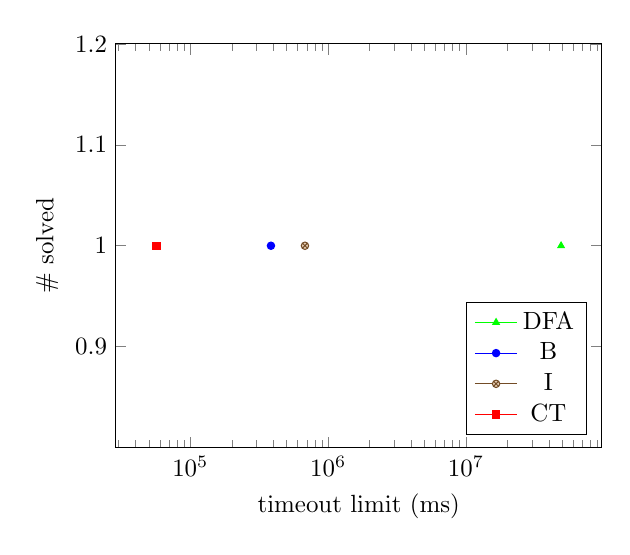
\begin{tikzpicture}[scale=0.9]
      \begin{axis}[
    xmode=log,
    every axis plot/.style={thin},
    xlabel={timeout limit (ms)},
    ylabel={\# solved},
    legend pos=south east
    % table/create on use/cumulative distribution/.style={
    %   create col/expr={\pgfmathaccuma + \thisrow{f(x)}}   
    % }
    ]
    \addplot 
    [mark=triangle*,
    mark size=1.5,
    mark options={solid},
    green] 
    coordinates {
    (48965354.632, 1)
    };

    \addplot 
    [blue,
    mark=*,
    mark size=1.5,
    mark options={solid}]
    coordinates {
    (384568.592, 1)
    };

    \addplot [brown!60!black,
    mark options={fill=brown!40},
    mark=otimes*,
    mark size=1.5]
    coordinates {
    (678711.642, 1)
    };

    \addplot 
    [red,
    mark size=1.5,
    mark=square*]
    coordinates {
    (56663.024, 1)
    };
    \legend{DFA,B,I,CT}
  \end{axis}

    \end{tikzpicture}
    \vfill
    \caption{\textbf{BDD Small}.}
    \vspace{\baselineskip}
  \end{minipage}\qquad
\end{figure}


\clearpage

\begin{figure}
  
  \begin{minipage}[b][10cm][s]{0.45\textwidth}
    \centering
    \vfill
    \begin{tikzpicture}[scale=0.9]
      \begin{axis}[
    xmode=log,
    every axis plot/.style={thin},
    xlabel={timeout limit (ms)},
    ylabel={\% solved},
    legend pos=south east,
    cycle list/Set1-6,
            % define fill color for the marker
            mark list fill={.!75!white},
            mark options={solid},
            cycle multiindex* list={
                Set1-6
                    \nextlist
                [3 of]linestyles
                    \nextlist
                very thick
                \nextlist
                mark=o,
                mark=*,
                mark=square,
                mark=triangle,
                mark=+
            },
    ]

    \addplot
    coordinates {
      (10, 100)
      
    };
    \addplot
    coordinates {
      (2410, 34)
      (4310, 67)
      (7220, 100)
      
    };
    \addplot
    coordinates {
      (3730, 34)
      (6480, 67)
      (11110, 100)
      
    };
    \addplot
    coordinates {
      (1780, 34)
      (2680, 67)
      (4360, 100)
      
    };
    

    \legend{ DFA, B, I, \textbf{CT} }
  \end{axis}

    \end{tikzpicture}
    \vfill
    \caption{\textbf{AIM-50}.}
    \vspace{\baselineskip}
  \end{minipage}\qquad
  \begin{minipage}[b][10cm][s]{0.45\textwidth}
    \centering
    \vfill
    \begin{tikzpicture}[scale=0.9]
      \begin{axis}[
    xmode=log,
    every axis plot/.style={thin},
    xlabel={timeout limit (ms)},
    ylabel={\% solved},
    legend style={at={(0.5,-0.30)},
      anchor=north,legend columns=-1},
    % legend pos=south east,
    cycle list/Set1-6,
            % define fill color for the marker
            mark list fill={.!75!white},
            mark options={solid,scale=0.9},
            cycle multiindex* list={
                Set1-6
                    \nextlist
                [3 of]linestyles
                    \nextlist
                very thick
                \nextlist
                mark=o,
                mark=*,
                mark=square,
                mark=triangle,
                mark=+
            },
    ]

    \addplot
    coordinates {
      (4710, 7)
      (42720, 14)
      (107940, 20)
      (156470, 27)
      (565750, 34)
      
    };
    \addplot
    coordinates {
      (4200, 7)
      (40280, 14)
      (101330, 20)
      (146750, 27)
      (542500, 34)
      
    };
    \addplot
    coordinates {
      (6700, 7)
      (64020, 14)
      (162760, 20)
      (236800, 27)
      (861730, 34)
      
    };
    \addplot
    coordinates {
      (5070, 7)
      (39550, 14)
      (103230, 20)
      (149210, 27)
      (482760, 34)
      
    };
    

    \legend{ DFA, B, I, \textbf{CT} }
  \end{axis}

    \end{tikzpicture}
    \vfill
    \caption{\textbf{AIM-100}.}
    \vspace{\baselineskip}
  \end{minipage}\qquad
\end{figure}

\begin{figure}
  \begin{minipage}[b][10cm][s]{0.45\textwidth}
    \centering
    \vfill
    \begin{tikzpicture}[scale=0.9]
      \begin{axis}[
    xmode=log,
    every axis plot/.style={thin},
    xlabel={timeout limit (ms)},
    ylabel={\% solved},
    legend pos=south east,
    cycle list/Set1-6,
            % define fill color for the marker
            mark list fill={.!75!white},
            mark options={solid},
            cycle multiindex* list={
                Set1-6
                    \nextlist
                [3 of]linestyles
                    \nextlist
                very thick
                \nextlist
                mark=o,
                mark=*,
                mark=square,
                mark=triangle,
                mark=+
            },
    ]

    \addplot
    coordinates {
      (5400, 5)
      (9950, 10)
      
    };
    \addplot
    coordinates {
      (4990, 5)
      (9390, 10)
      
    };
    \addplot
    coordinates {
      (7850, 5)
      (14800, 10)
      
    };
    \addplot
    coordinates {
      (6840, 5)
      (12750, 10)
      
    };
    

    \legend{ DFA, B, I, \textbf{CT} }
  \end{axis}

    \end{tikzpicture}
    \vfill
    \caption{\textbf{AIM-200}.}
    \vspace{\baselineskip}
  \end{minipage}\qquad
\end{figure}


\clearpage

\begin{figure}
  \begin{minipage}[b][10cm][s]{0.45\textwidth}
    \centering
    \vfill
    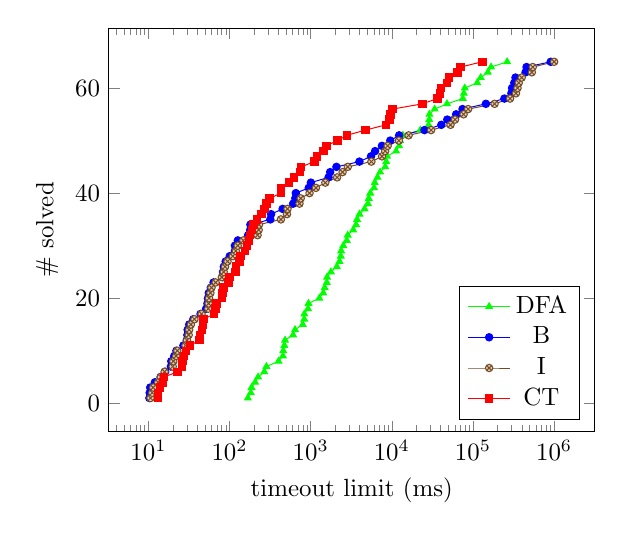
\begin{tikzpicture}[scale=0.9]
      \begin{axis}[
    xmode=log,
    every axis plot/.style={thin},
    xlabel={timeout limit (ms)},
    ylabel={\# solved},
    legend pos=south east
    % table/create on use/cumulative distribution/.style={
    %   create col/expr={\pgfmathaccuma + \thisrow{f(x)}}   
    % }
    ]
    \addplot 
    [mark=triangle*,
    mark size=1.5,
    mark options={solid},
    green] 
    coordinates {
    (168.150, 1)
(182.863, 2)
(186.751, 3)
(206.978, 4)
(224.861, 5)
(268.023, 6)
(284.689, 7)
(401.351, 8)
(455.154, 9)
(459.206, 10)
(473.618, 11)
(482.924, 12)
(606.837, 13)
(641.324, 14)
(798.435, 15)
(832.510, 16)
(835.157, 17)
(928.392, 18)
(940.176, 19)
(1277.548, 20)
(1428.508, 21)
(1489.070, 22)
(1578.965, 23)
(1591.384, 24)
(1774.863, 25)
(2099.680, 26)
(2263.069, 27)
(2348.325, 28)
(2373.974, 29)
(2520.594, 30)
(2784.923, 31)
(2861.514, 32)
(3342.441, 33)
(3631.192, 34)
(3731.033, 35)
(3990.165, 36)
(4612.172, 37)
(5065.103, 38)
(5196.760, 39)
(5422.844, 40)
(6036.793, 41)
(6158.096, 42)
(6651.780, 43)
(7172.739, 44)
(8299.992, 45)
(8527.100, 46)
(8742.155, 47)
(11283.274, 48)
(12311.489, 49)
(12691.810, 50)
(13696.709, 51)
(22444.918, 52)
(28416.398, 53)
(28898.843, 54)
(29066.696, 55)
(33716.949, 56)
(47818.922, 57)
(75088.099, 58)
(77218.417, 59)
(79265.402, 60)
(112886.647, 61)
(124665.719, 62)
(152476.582, 63)
(167086.736, 64)
(263675.831, 65)
    };

    \addplot 
    [blue,
    mark=*,
    mark size=1.5,
    mark options={solid}]
    coordinates {
    (10.288, 1)
(10.379, 2)
(10.535, 3)
(12.034, 4)
(14.149, 5)
(16.100, 6)
(18.933, 7)
(19.139, 8)
(20.839, 9)
(22.139, 10)
(27.012, 11)
(29.711, 12)
(30.231, 13)
(30.470, 14)
(31.870, 15)
(35.827, 16)
(43.904, 17)
(51.491, 18)
(53.414, 19)
(54.245, 20)
(55.529, 21)
(58.813, 22)
(63.560, 23)
(82.820, 24)
(83.059, 25)
(84.984, 26)
(89.582, 27)
(100.635, 28)
(116.336, 29)
(116.387, 30)
(126.573, 31)
(169.492, 32)
(179.688, 33)
(180.688, 34)
(318.127, 35)
(325.169, 36)
(451.143, 37)
(607.991, 38)
(646.090, 39)
(656.228, 40)
(946.080, 41)
(1004.658, 42)
(1660.359, 43)
(1737.596, 44)
(2076.743, 45)
(3987.950, 46)
(5535.172, 47)
(6216.507, 48)
(7553.621, 49)
(9566.318, 50)
(12314.159, 51)
(25255.025, 52)
(40714.988, 53)
(48185.890, 54)
(62038.155, 55)
(74358.984, 56)
(144199.158, 57)
(243953.168, 58)
(297058.443, 59)
(303002.147, 60)
(322643.726, 61)
(334099.524, 62)
(444760.548, 63)
(457245.676, 64)
(908299.991, 65)
    };

    \addplot [brown!60!black,
    mark options={fill=brown!40},
    mark=otimes*,
    mark size=1.5]
    coordinates {
    (10.616, 1)
(11.157, 2)
(11.450, 3)
(13.215, 4)
(14.216, 5)
(15.849, 6)
(19.947, 7)
(20.281, 8)
(22.000, 9)
(22.742, 10)
(28.631, 11)
(29.926, 12)
(31.370, 13)
(31.817, 14)
(33.408, 15)
(36.961, 16)
(45.187, 17)
(54.697, 18)
(55.264, 19)
(55.881, 20)
(58.129, 21)
(59.930, 22)
(67.399, 23)
(80.411, 24)
(84.715, 25)
(88.104, 26)
(94.466, 27)
(109.734, 28)
(119.623, 29)
(126.131, 30)
(147.816, 31)
(221.417, 32)
(228.637, 33)
(230.714, 34)
(429.542, 35)
(510.620, 36)
(518.047, 37)
(727.879, 38)
(753.405, 39)
(967.759, 40)
(1160.759, 41)
(1515.104, 42)
(2117.217, 43)
(2471.293, 44)
(2864.755, 45)
(5598.516, 46)
(7567.878, 47)
(8280.206, 48)
(8880.976, 49)
(12216.638, 50)
(16096.927, 51)
(30488.085, 52)
(52877.821, 53)
(60162.558, 54)
(76670.942, 55)
(87192.459, 56)
(184694.430, 57)
(286473.826, 58)
(338668.570, 59)
(353987.670, 60)
(366776.798, 61)
(398536.291, 62)
(531367.016, 63)
(545291.340, 64)
(1000123.027, 65)
    };

    \addplot 
    [red,
    mark size=1.5,
    mark=square*]
    coordinates {
    (13.060, 1)
(13.134, 2)
(13.813, 3)
(15.189, 4)
(15.583, 5)
(22.986, 6)
(25.913, 7)
(26.225, 8)
(27.291, 9)
(29.241, 10)
(32.661, 11)
(42.404, 12)
(43.556, 13)
(45.518, 14)
(47.353, 15)
(47.802, 16)
(64.076, 17)
(67.168, 18)
(69.160, 19)
(80.841, 20)
(81.435, 21)
(84.476, 22)
(97.192, 23)
(100.374, 24)
(118.778, 25)
(119.779, 26)
(132.448, 27)
(136.798, 28)
(154.350, 29)
(164.133, 30)
(173.260, 31)
(178.961, 32)
(188.870, 33)
(198.624, 34)
(219.567, 35)
(246.380, 36)
(268.687, 37)
(286.696, 38)
(311.978, 39)
(428.872, 40)
(431.630, 41)
(537.920, 42)
(621.376, 43)
(734.095, 44)
(762.025, 45)
(1111.200, 46)
(1200.228, 47)
(1447.420, 48)
(1558.032, 49)
(2135.953, 50)
(2786.377, 51)
(4721.767, 52)
(8456.834, 53)
(9396.061, 54)
(9677.141, 55)
(10197.232, 56)
(23825.877, 57)
(36319.204, 58)
(38988.650, 59)
(40323.398, 60)
(47704.623, 61)
(50664.686, 62)
(64490.153, 63)
(70365.144, 64)
(130202.335, 65)
    };
    \legend{DFA,B,I,CT}
  \end{axis}

    \end{tikzpicture}
    \vfill
    \caption{\textbf{Crosswords WorldVG}.}
    \vspace{\baselineskip}
  \end{minipage}\qquad
  \begin{minipage}[b][10cm][s]{0.45\textwidth}
    \centering
    \vfill
    \begin{tikzpicture}[scale=0.9]
      \begin{axis}[
    xmode=log,
    every axis plot/.style={thin},
    xlabel={timeout limit (ms)},
    ylabel={\% solved},
    legend pos=south east,
    cycle list/Set1-6,
            % define fill color for the marker
            mark list fill={.!75!white},
            mark options={solid},
            cycle multiindex* list={
                Set1-6
                    \nextlist
                [3 of]linestyles
                    \nextlist
                very thick
                \nextlist
                mark=o,
                mark=*,
                mark=square,
                mark=triangle,
                mark=+
            },
    ]

    \addplot
    coordinates {
      (770, 4)
      (1030, 7)
      (1190, 10)
      (1460, 13)
      (1480, 16)
      (1610, 19)
      (1650, 22)
      (2100, 28)
      (2220, 31)
      (2290, 34)
      (3030, 37)
      (3050, 40)
      (3200, 43)
      (3210, 46)
      (3940, 49)
      (4820, 52)
      (5510, 55)
      (5960, 58)
      (6580, 61)
      (8120, 64)
      (12080, 67)
      (13060, 70)
      (14920, 73)
      (15710, 76)
      (19260, 79)
      (22550, 82)
      (29920, 85)
      (35600, 88)
      (36330, 91)
      (54060, 94)
      (60090, 97)
      (76370, 100)
      
    };
    \addplot
    coordinates {
      (60, 4)
      (70, 7)
      (80, 10)
      (90, 13)
      (130, 19)
      (200, 22)
      (240, 25)
      (330, 28)
      (360, 31)
      (840, 34)
      (1000, 37)
      (1340, 40)
      (1430, 43)
      (1550, 46)
      (2540, 49)
      (2810, 52)
      (4430, 55)
      (5340, 58)
      (7400, 61)
      (7450, 64)
      (12980, 67)
      (16570, 70)
      (19500, 73)
      (20590, 76)
      (23780, 79)
      (38770, 82)
      (63540, 85)
      (66170, 88)
      (72660, 91)
      (111260, 94)
      (121100, 97)
      (144690, 100)
      
    };
    \addplot
    coordinates {
      (70, 7)
      (100, 13)
      (170, 16)
      (190, 19)
      (300, 22)
      (330, 25)
      (500, 28)
      (510, 31)
      (1130, 34)
      (1330, 37)
      (1620, 40)
      (1720, 43)
      (2180, 46)
      (3390, 49)
      (3680, 52)
      (5660, 55)
      (6820, 58)
      (9260, 61)
      (9470, 64)
      (16340, 67)
      (19480, 70)
      (24380, 73)
      (26140, 76)
      (29480, 79)
      (47910, 82)
      (75650, 85)
      (82650, 88)
      (87290, 91)
      (130370, 94)
      (140830, 97)
      (170720, 100)
      
    };
    \addplot
    coordinates {
      (60, 4)
      (70, 7)
      (80, 13)
      (100, 16)
      (110, 22)
      (140, 25)
      (160, 28)
      (180, 31)
      (220, 34)
      (230, 37)
      (250, 40)
      (290, 43)
      (430, 46)
      (510, 49)
      (560, 52)
      (810, 55)
      (940, 58)
      (1250, 61)
      (1270, 64)
      (2030, 67)
      (2410, 70)
      (2990, 73)
      (3290, 76)
      (3870, 79)
      (5870, 82)
      (10460, 85)
      (10710, 88)
      (11000, 91)
      (14610, 94)
      (19780, 97)
      (23710, 100)
      
    };
    

    \legend{ DFA, B, I, \textbf{CT} }
  \end{axis}

    \end{tikzpicture}
    \vfill
    \caption{\textbf{Crosswords LexVG}.}
    \vspace{\baselineskip}
  \end{minipage}\qquad
\end{figure}

\begin{figure}
  \begin{minipage}[b][10cm][s]{0.45\textwidth}
    \centering
    \vfill
    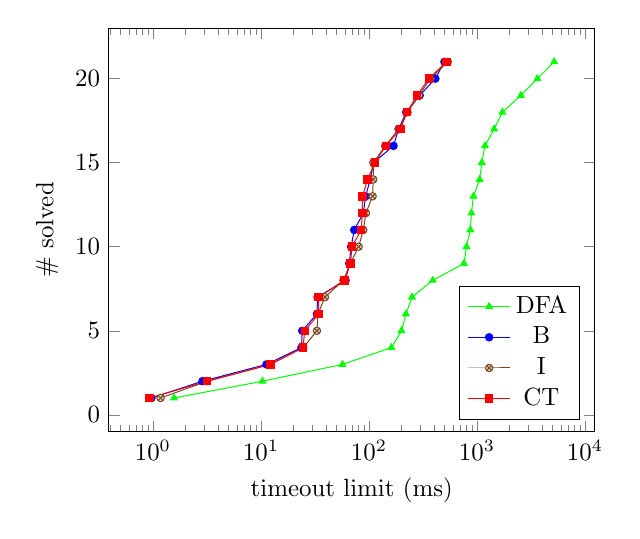
\begin{tikzpicture}[scale=0.9]
      \begin{axis}[
    xmode=log,
    every axis plot/.style={thin},
    xlabel={timeout limit (ms)},
    ylabel={\# solved},
    legend pos=south east
    % table/create on use/cumulative distribution/.style={
    %   create col/expr={\pgfmathaccuma + \thisrow{f(x)}}   
    % }
    ]
    \addplot 
    [mark=triangle*,
    mark size=1.5,
    mark options={solid},
    green] 
    coordinates {
(1.569, 1)
(10.341, 2)
(56.930, 3)
(161.466, 4)
(200.271, 5)
(220.150, 6)
(250.496, 7)
(389.479, 8)
(757.830, 9)
(800.580, 10)
(868.873, 11)
(888.415, 12)
(928.329, 13)
(1059.826, 14)
(1108.592, 15)
(1186.171, 16)
(1442.143, 17)
(1718.117, 18)
(2549.019, 19)
(3626.036, 20)
(5178.601, 21)
    };

    \addplot 
    [blue,
    mark=*,
    mark size=1.5,
    mark options={solid}]
    coordinates {
(0.969, 1)
(2.881, 2)
(11.268, 3)
(23.734, 4)
(24.138, 5)
(33.016, 6)
(33.480, 7)
(60.819, 8)
(65.730, 9)
(68.464, 10)
(73.136, 11)
(88.944, 12)
(92.941, 13)
(103.030, 14)
(110.307, 15)
(168.815, 16)
(188.304, 17)
(221.341, 18)
(295.291, 19)
(412.154, 20)
(499.695, 21)
    };

    \addplot [brown!60!black,
    mark options={fill=brown!40},
    mark=otimes*,
    mark size=1.5]
    coordinates {
(1.178, 1)
(3.182, 2)
(12.190, 3)
(24.682, 4)
(33.012, 5)
(33.778, 6)
(39.197, 7)
(58.045, 8)
(67.182, 9)
(80.311, 10)
(88.742, 11)
(93.862, 12)
(108.193, 13)
(109.575, 14)
(110.207, 15)
(141.416, 16)
(189.383, 17)
(227.490, 18)
(289.981, 19)
(370.487, 20)
(537.222, 21)
    };

    \addplot 
    [red,
    mark size=1.5,
    mark=square*]
    coordinates {
(0.929, 1)
(3.171, 2)
(12.289, 3)
(24.504, 4)
(25.467, 5)
(34.223, 6)
(34.294, 7)
(59.192, 8)
(67.660, 9)
(69.445, 10)
(84.905, 11)
(86.923, 12)
(87.166, 13)
(97.317, 14)
(113.314, 15)
(143.394, 16)
(195.333, 17)
(225.252, 18)
(279.125, 19)
(358.324, 20)
(525.028, 21)
    };
    \legend{DFA,B,I,CT}
  \end{axis}

    \end{tikzpicture}
    \vfill
    \caption{\textbf{Crosswords Wordspuzzle}.}
    \vspace{\baselineskip}
  \end{minipage}\qquad
\end{figure}


\clearpage

\begin{figure}
  \begin{minipage}[b][10cm][s]{0.45\textwidth}
    \centering
    \vfill
    \begin{tikzpicture}[scale=0.9]
      \begin{axis}[
    xmode=log,
    every axis plot/.style={thin},
    xlabel={timeout limit (ms)},
    ylabel={\% solved},
    legend pos=south east,
    cycle list/Set1-6,
            % define fill color for the marker
            mark list fill={.!75!white},
            mark options={solid},
            cycle multiindex* list={
                Set1-6
                    \nextlist
                [3 of]linestyles
                    \nextlist
                very thick
                \nextlist
                mark=o,
                mark=*,
                mark=square,
                mark=triangle,
                mark=+
            },
    ]

    \addplot
    coordinates {
      (25170, 8)
      (52050, 16)
      (106800, 24)
      (221140, 31)
      (461470, 39)
      (939670, 47)
      
    };
    \addplot
    coordinates {
      (23990, 8)
      (50380, 16)
      (105170, 24)
      (215170, 31)
      (449310, 39)
      (925510, 47)
      
    };
    \addplot
    coordinates {
      (32120, 8)
      (65960, 16)
      (137030, 24)
      (282220, 31)
      (583270, 39)
      
    };
    \addplot
    coordinates {
      (22530, 8)
      (46610, 16)
      (96430, 24)
      (198370, 31)
      (409390, 39)
      (855630, 47)
      
    };
    

    \legend{ DFA, B, I, \textbf{CT} }
  \end{axis}

    \end{tikzpicture}
    \vfill
    \caption{\textbf{Dubois}.}
    \vspace{\baselineskip}
  \end{minipage}\qquad
  \begin{minipage}[b][10cm][s]{0.45\textwidth}
    \centering
    \vfill
    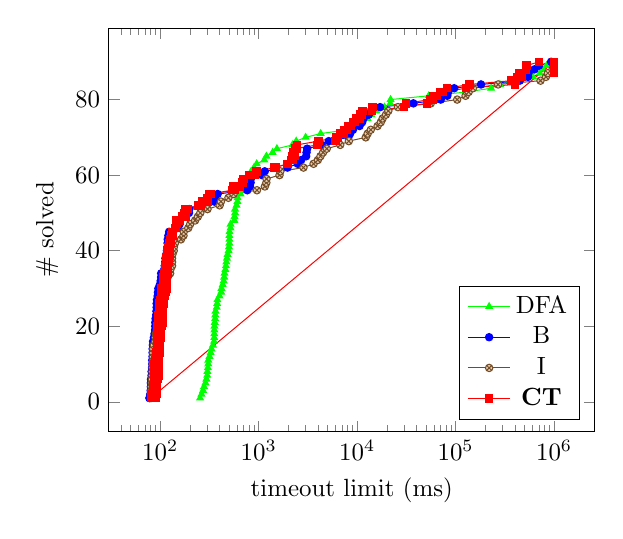
\begin{tikzpicture}[scale=0.9]
      \begin{axis}[
    xmode=log,
    every axis plot/.style={thin},
    xlabel={timeout limit (ms)},
    ylabel={\# solved},
    legend pos=south east
    % table/create on use/cumulative distribution/.style={
    %   create col/expr={\pgfmathaccuma + \thisrow{f(x)}}   
    % }
    ]
    \addplot 
    [mark=triangle*,
    mark size=1.5,
    mark options={solid},
    green] 
    coordinates {
(253.940, 1)
(262.899, 2)
(272.809, 3)
(278.671, 4)
(288.456, 5)
(294.738, 6)
(300.533, 7)
(301.856, 8)
(305.317, 9)
(307.585, 10)
(307.747, 11)
(317.045, 12)
(325.386, 13)
(331.714, 14)
(343.719, 15)
(352.611, 16)
(354.157, 17)
(354.187, 18)
(355.194, 19)
(355.670, 20)
(358.353, 21)
(361.624, 22)
(363.056, 23)
(364.990, 24)
(375.254, 25)
(379.066, 26)
(381.267, 27)
(400.323, 28)
(416.524, 29)
(419.193, 30)
(431.537, 31)
(441.410, 32)
(446.582, 33)
(449.777, 34)
(459.308, 35)
(465.151, 36)
(469.990, 37)
(476.800, 38)
(483.769, 39)
(495.431, 40)
(499.645, 41)
(504.063, 42)
(504.308, 43)
(504.525, 44)
(505.961, 45)
(518.392, 46)
(518.507, 47)
(566.413, 48)
(568.752, 49)
(575.921, 50)
(576.168, 51)
(596.357, 52)
(608.960, 53)
(610.697, 54)
(655.605, 55)
(657.724, 56)
(659.099, 57)
(661.565, 58)
(793.731, 59)
(829.897, 60)
(838.681, 61)
(897.103, 62)
(955.465, 63)
(1140.095, 64)
(1197.349, 65)
(1386.206, 66)
(1532.332, 67)
(2202.746, 68)
(2405.914, 69)
(2998.076, 70)
(4263.504, 71)
(7966.854, 72)
(8986.821, 73)
(10565.606, 74)
(12775.906, 75)
(13934.651, 76)
(15637.959, 77)
(18950.571, 78)
(21686.565, 79)
(21854.085, 80)
(53338.868, 81)
(128675.786, 82)
(229123.808, 83)
(281459.430, 84)
(391898.437, 85)
(610230.975, 86)
(714999.649, 87)
(762531.311, 88)
(838054.743, 89)
    };

    \addplot 
    [blue,
    mark=*,
    mark size=1.5,
    mark options={solid}]
    coordinates {
(77.750, 1)
(79.361, 2)
(80.110, 3)
(80.478, 4)
(80.514, 5)
(80.733, 6)
(81.819, 7)
(81.865, 8)
(82.700, 9)
(83.055, 10)
(83.084, 11)
(83.660, 12)
(83.815, 13)
(83.884, 14)
(84.339, 15)
(84.779, 16)
(86.333, 17)
(87.672, 18)
(88.800, 19)
(89.170, 20)
(89.209, 21)
(89.917, 22)
(91.234, 23)
(91.710, 24)
(92.131, 25)
(92.191, 26)
(92.825, 27)
(94.385, 28)
(94.984, 29)
(95.858, 30)
(99.363, 31)
(101.208, 32)
(102.326, 33)
(102.457, 34)
(109.924, 35)
(111.293, 36)
(112.684, 37)
(113.090, 38)
(115.314, 39)
(117.192, 40)
(118.738, 41)
(118.994, 42)
(119.411, 43)
(121.235, 44)
(123.390, 45)
(150.523, 46)
(157.344, 47)
(158.315, 48)
(182.842, 49)
(196.164, 50)
(197.579, 51)
(277.635, 52)
(354.634, 53)
(359.251, 54)
(383.268, 55)
(766.566, 56)
(816.221, 57)
(827.832, 58)
(833.240, 59)
(1081.574, 60)
(1153.362, 61)
(1963.070, 62)
(2492.142, 63)
(2701.259, 64)
(3034.945, 65)
(3062.028, 66)
(3107.310, 67)
(4356.706, 68)
(5152.815, 69)
(8143.306, 70)
(8488.009, 71)
(9065.789, 72)
(10578.592, 73)
(11242.491, 74)
(11618.200, 75)
(13121.563, 76)
(13946.231, 77)
(17115.205, 78)
(37255.008, 79)
(70596.495, 80)
(82332.599, 81)
(83994.429, 82)
(96686.082, 83)
(180912.619, 84)
(447647.179, 85)
(543188.377, 86)
(549287.562, 87)
(631674.574, 88)
(702660.342, 89)
(931931.366, 90)
    };

    \addplot [brown!60!black,
    mark options={fill=brown!40},
    mark=otimes*,
    mark size=1.5]
    coordinates {
(80.607, 1)
(80.621, 2)
(81.289, 3)
(81.598, 4)
(81.969, 5)
(82.414, 6)
(83.447, 7)
(83.492, 8)
(83.796, 9)
(83.946, 10)
(84.672, 11)
(84.778, 12)
(84.834, 13)
(85.069, 14)
(86.207, 15)
(89.293, 16)
(89.663, 17)
(90.436, 18)
(92.701, 19)
(93.412, 20)
(95.453, 21)
(96.026, 22)
(97.734, 23)
(99.208, 24)
(101.597, 25)
(103.239, 26)
(103.380, 27)
(103.698, 28)
(107.856, 29)
(109.858, 30)
(111.092, 31)
(116.012, 32)
(119.197, 33)
(126.351, 34)
(126.923, 35)
(131.997, 36)
(132.037, 37)
(132.076, 38)
(133.087, 39)
(137.356, 40)
(137.793, 41)
(141.326, 42)
(162.716, 43)
(172.556, 44)
(173.424, 45)
(192.918, 46)
(201.428, 47)
(226.385, 48)
(241.352, 49)
(255.602, 50)
(302.351, 51)
(401.666, 52)
(413.952, 53)
(493.052, 54)
(555.383, 55)
(961.003, 56)
(1155.835, 57)
(1196.833, 58)
(1202.095, 59)
(1628.244, 60)
(1659.941, 61)
(2850.318, 62)
(3611.710, 63)
(3991.524, 64)
(4242.800, 65)
(4511.471, 66)
(4915.881, 67)
(6733.256, 68)
(8232.380, 69)
(12233.495, 70)
(12792.050, 71)
(13747.597, 72)
(16126.327, 73)
(17376.344, 74)
(18154.073, 75)
(19607.670, 76)
(20742.169, 77)
(25931.910, 78)
(55946.249, 79)
(103693.950, 80)
(126173.635, 81)
(135526.885, 82)
(149917.691, 83)
(270068.501, 84)
(727604.821, 85)
(825691.112, 86)
(863292.217, 87)
(964034.894, 88)
    };

    \addplot 
    [red,
    mark size=1.5,
    mark=square*]
    coordinates {
    (89.550, 1)
(91.628, 2)
(91.874, 3)
(91.916, 4)
(92.882, 5)
(95.582, 6)
(96.208, 7)
(96.305, 8)
(96.355, 9)
(96.836, 10)
(97.104, 11)
(97.774, 12)
(98.219, 13)
(98.842, 14)
(99.086, 15)
(99.460, 16)
(101.107, 17)
(101.569, 18)
(101.733, 19)
(103.618, 20)
(105.602, 21)
(105.708, 22)
(105.931, 23)
(105.945, 24)
(106.654, 25)
(108.520, 26)
(108.809, 27)
(112.070, 28)
(114.845, 29)
(117.067, 30)
(117.306, 31)
(117.414, 32)
(117.677, 33)
(118.388, 34)
(118.836, 35)
(119.381, 36)
(120.948, 37)
(122.430, 38)
(124.161, 39)
(124.606, 40)
(126.364, 41)
(126.885, 42)
(127.749, 43)
(133.597, 44)
(134.258, 45)
(143.320, 46)
(146.695, 47)
(156.485, 48)
(182.731, 49)
(183.424, 50)
(189.376, 51)
(261.174, 52)
(267.469, 53)
(300.773, 54)
(313.223, 55)
(536.125, 56)
(550.835, 57)
(691.130, 58)
(695.096, 59)
(809.479, 60)
(952.531, 61)
(1448.230, 62)
(1953.052, 63)
(2147.694, 64)
(2183.764, 65)
(2243.511, 66)
(2365.130, 67)
(3960.400, 68)
(6032.483, 69)
(6405.844, 70)
(7301.289, 71)
(7824.570, 72)
(8664.157, 73)
(9497.544, 74)
(10520.711, 75)
(11028.497, 76)
(14183.925, 77)
(29834.289, 78)
(51033.896, 79)
(58889.443, 80)
(59117.236, 81)
(73470.919, 82)
(127470.124, 83)
(398914.967, 84)
(405525.944, 85)
(466311.297, 86)
(1000113.581, 87)
(1000121.152, 88)
(1000123.083, 89)
(1000137.593, 90)
(80.539, 1)
(82.933, 2)
(84.502, 3)
(85.194, 4)
(86.750, 5)
(87.225, 6)
(87.348, 7)
(87.379, 8)
(87.590, 9)
(87.799, 10)
(89.072, 11)
(90.371, 12)
(91.497, 13)
(92.339, 14)
(92.677, 15)
(92.786, 16)
(92.837, 17)
(93.306, 18)
(94.022, 19)
(94.387, 20)
(94.732, 21)
(94.876, 22)
(95.771, 23)
(97.088, 24)
(97.931, 25)
(98.786, 26)
(99.264, 27)
(101.340, 28)
(102.067, 29)
(102.698, 30)
(106.996, 31)
(108.150, 32)
(108.319, 33)
(109.028, 34)
(112.687, 35)
(112.838, 36)
(113.987, 37)
(115.735, 38)
(116.607, 39)
(117.896, 40)
(120.281, 41)
(124.525, 42)
(127.605, 43)
(129.317, 44)
(131.451, 45)
(140.940, 46)
(144.202, 47)
(145.438, 48)
(168.774, 49)
(174.703, 50)
(178.916, 51)
(244.908, 52)
(305.799, 53)
(306.522, 54)
(329.051, 55)
(577.969, 56)
(639.964, 57)
(687.996, 58)
(705.323, 59)
(904.996, 60)
(941.051, 61)
(1495.517, 62)
(1970.419, 63)
(2227.812, 64)
(2340.143, 65)
(2350.643, 66)
(2430.290, 67)
(2443.247, 68)
(4040.442, 69)
(6139.544, 70)
(6717.200, 71)
(7384.930, 72)
(8139.677, 73)
(9195.984, 74)
(9860.741, 75)
(10763.986, 76)
(11275.949, 77)
(14355.361, 78)
(31179.882, 79)
(55057.738, 80)
(64542.114, 81)
(70093.034, 82)
(81511.901, 83)
(138808.782, 84)
(367231.073, 85)
(417571.146, 86)
(437364.064, 87)
(519365.523, 88)
(525638.664, 89)
(705868.408, 90)
    };
    \legend{DFA,B,I,\textbf{CT}}
  \end{axis}

    \end{tikzpicture}
    \vfill
    \caption{\textbf{Geom}.}
    \vspace{\baselineskip}
  \end{minipage}\qquad
\end{figure}

\begin{figure}
  \begin{minipage}[b][10cm][s]{0.45\textwidth}
    \centering
    \vfill
    \begin{tikzpicture}[scale=0.9]
      \begin{axis}[
    xmode=log,
    every axis plot/.style={thin},
    xlabel={timeout limit (ms)},
    ylabel={\% solved},
    legend style={at={(0.5,-0.30)},
      anchor=north,legend columns=-1},
    % legend pos=south east,
    cycle list/Set1-6,
            % define fill color for the marker
            mark list fill={.!75!white},
            mark options={solid,scale=0.9},
            cycle multiindex* list={
                Set1-6
                    \nextlist
                [3 of]linestyles
                    \nextlist
                very thick
                \nextlist
                mark=o,
                mark=*,
                mark=square,
                mark=triangle,
                mark=+
            },
    ]

    \addplot
    coordinates {
      (8240, 10)
      (8300, 20)
      (8800, 30)
      (9050, 40)
      (11550, 50)
      (14490, 60)
      (15490, 70)
      (15680, 80)
      (16230, 90)
      (17510, 100)
      
    };
    \addplot
    coordinates {
      (8710, 10)
      (13000, 20)
      (16840, 30)
      (17370, 40)
      (19860, 50)
      (28430, 60)
      (31470, 70)
      (41080, 80)
      (46790, 90)
      (48720, 100)
      
    };
    \addplot
    coordinates {
      (9810, 10)
      (12550, 20)
      (19300, 30)
      (20370, 40)
      (21220, 50)
      (33870, 60)
      (34700, 70)
      (47590, 80)
      (49800, 90)
      (50780, 100)
      
    };
    \addplot
    coordinates {
      (1180, 10)
      (1220, 20)
      (1700, 30)
      (1880, 40)
      (1940, 50)
      (2860, 60)
      (3050, 70)
      (3140, 80)
      (3860, 90)
      (4150, 100)
      
    };
    

    \legend{ DFA, B, I, \textbf{CT} }
  \end{axis}

    \end{tikzpicture}
    \vfill
    \caption{\textbf{K5}.}
    \vspace{\baselineskip}
  \end{minipage}\qquad
\end{figure}

\clearpage

\begin{figure}
  \begin{minipage}[b][10cm][s]{0.45\textwidth}
    \centering
    \vfill
    \begin{tikzpicture}[scale=0.9]
      \begin{axis}[
    xmode=log,
    every axis plot/.style={thin},
    xlabel={timeout limit (ms)},
    ylabel={\% solved},
    legend pos=south east,
    cycle list/Set1-6,
            % define fill color for the marker
            mark list fill={.!75!white},
            mark options={solid},
            cycle multiindex* list={
                Set1-6
                    \nextlist
                [3 of]linestyles
                    \nextlist
                very thick
                \nextlist
                mark=o,
                mark=*,
                mark=square,
                mark=triangle,
                mark=+
            },
    ]

    \addplot
    coordinates {
      (1030, 8)
      (1170, 16)
      (1970, 24)
      (2380, 31)
      (2400, 39)
      (2430, 47)
      (3000, 54)
      (3350, 62)
      (3400, 70)
      (4590, 77)
      (4870, 85)
      (5590, 93)
      (6420, 100)
      
    };
    \addplot
    coordinates {
      (160, 8)
      (180, 16)
      (220, 24)
      (250, 47)
      (270, 54)
      (310, 62)
      (340, 70)
      (430, 77)
      (440, 85)
      (530, 93)
      (560, 100)
      
    };
    \addplot
    coordinates {
      (160, 8)
      (180, 16)
      (220, 24)
      (250, 47)
      (270, 54)
      (310, 62)
      (340, 70)
      (430, 77)
      (440, 85)
      (540, 93)
      (560, 100)
      
    };
    \addplot
    coordinates {
      (160, 8)
      (180, 16)
      (230, 24)
      (240, 31)
      (250, 47)
      (270, 54)
      (310, 62)
      (340, 70)
      (440, 85)
      (540, 93)
      (550, 100)
      
    };
    

    \legend{ DFA, B, I, \textbf{CT} }
  \end{axis}

    \end{tikzpicture}
    \vfill
    \caption{\textbf{Kakuro easy}.}
    \vspace{\baselineskip}
  \end{minipage}\qquad
  \begin{minipage}[b][10cm][s]{0.45\textwidth}
    \centering
    \vfill
    \begin{tikzpicture}[scale=0.9]
      \begin{axis}[
    xmode=log,
    every axis plot/.style={thin},
    xlabel={timeout limit (ms)},
    ylabel={\% solved},
    legend pos=south east,
    cycle list/Set1-6,
            % define fill color for the marker
            mark list fill={.!75!white},
            mark options={solid},
            cycle multiindex* list={
                Set1-6
                    \nextlist
                [3 of]linestyles
                    \nextlist
                very thick
                \nextlist
                mark=o,
                mark=*,
                mark=square,
                mark=triangle,
                mark=+
            },
    ]

    \addplot
    coordinates {
      (1740, 7)
      (2370, 14)
      (2440, 27)
      (3030, 40)
      (3070, 47)
      (3500, 54)
      (4640, 60)
      (4670, 67)
      (4940, 74)
      (5240, 80)
      (5930, 87)
      (6460, 94)
      (7430, 100)
      
    };
    \addplot
    coordinates {
      (210, 3)
      (250, 10)
      (270, 12)
      (360, 14)
      (370, 16)
      (380, 19)
      (470, 21)
      (500, 23)
      (540, 25)
      (550, 28)
      (580, 30)
      (630, 32)
      (690, 35)
      (1640, 37)
      (1820, 39)
      (2070, 41)
      (2300, 44)
      (2410, 46)
      (2560, 50)
      (2640, 53)
      (2850, 55)
      (3010, 57)
      (3200, 60)
      (3640, 62)
      (3700, 64)
      (3840, 66)
      (3950, 69)
      (3960, 71)
      (3980, 73)
      (4050, 75)
      (4480, 78)
      (4880, 80)
      (5000, 82)
      (5060, 85)
      (5420, 87)
      (5740, 89)
      (5900, 91)
      (8200, 94)
      (8640, 96)
      (10020, 98)
      (12650, 100)
      
    };
    \addplot
    coordinates {
      (220, 3)
      (250, 5)
      (260, 10)
      (270, 12)
      (340, 14)
      (360, 16)
      (380, 19)
      (470, 21)
      (490, 23)
      (540, 28)
      (580, 30)
      (630, 32)
      (690, 35)
      (1130, 37)
      (1170, 39)
      (1220, 41)
      (1850, 46)
      (1860, 48)
      (1870, 50)
      (1900, 53)
      (2080, 55)
      (2120, 57)
      (2170, 60)
      (2230, 62)
      (2460, 64)
      (2650, 66)
      (3310, 69)
      (3330, 71)
      (3350, 73)
      (3370, 75)
      (3430, 78)
      (3590, 80)
      (4130, 82)
      (4810, 85)
      (4920, 87)
      (4950, 89)
      (4980, 91)
      (7810, 94)
      (7850, 96)
      (10570, 98)
      (12030, 100)
      
    };
    \addplot
    coordinates {
      (210, 3)
      (250, 5)
      (260, 10)
      (280, 12)
      (340, 14)
      (360, 16)
      (390, 19)
      (470, 21)
      (500, 23)
      (550, 28)
      (590, 30)
      (620, 32)
      (700, 35)
      (1120, 37)
      (1150, 39)
      (1200, 41)
      (1820, 44)
      (1830, 46)
      (1880, 50)
      (1890, 53)
      (2100, 55)
      (2130, 57)
      (2200, 60)
      (2220, 62)
      (2450, 64)
      (2650, 66)
      (3320, 69)
      (3330, 71)
      (3370, 73)
      (3400, 75)
      (3470, 78)
      (3500, 80)
      (4060, 82)
      (4800, 85)
      (4930, 89)
      (5050, 91)
      (7820, 94)
      (7950, 96)
      (9310, 98)
      (10850, 100)
      
    };
    

    \legend{ DFA, B, I, \textbf{CT} }
  \end{axis}

    \end{tikzpicture}
    \vfill
    \caption{\textbf{Kakuro Medium}.}
    \vspace{\baselineskip}
  \end{minipage}\qquad
\end{figure}


\begin{figure}
  \begin{minipage}[b][10cm][s]{0.45\textwidth}
    \centering
    \vfill
    \begin{tikzpicture}[scale=0.9]
      \begin{axis}[
    xmode=log,
    every axis plot/.style={thin},
    xlabel={timeout limit (ms)},
    ylabel={\% solved},
    legend style={at={(0.5,-0.30)},
      anchor=north,legend columns=-1},
    % legend pos=south east,
    cycle list/Set1-6,
            % define fill color for the marker
            mark list fill={.!75!white},
            mark options={solid,scale=0.9},
            cycle multiindex* list={
                Set1-6
                    \nextlist
                [3 of]linestyles
                    \nextlist
                very thick
                \nextlist
                mark=o,
                mark=*,
                mark=square,
                mark=triangle,
                mark=+
            },
    ]

    \addplot
    coordinates {
      (1030, 8)
      (2420, 16)
      (2630, 24)
      (2760, 31)
      (2910, 39)
      (3260, 47)
      (3700, 54)
      (4820, 62)
      (5260, 70)
      (5970, 77)
      (6170, 85)
      (6400, 93)
      (6620, 100)
      
    };
    \addplot
    coordinates {
      (170, 8)
      (240, 16)
      (260, 24)
      (290, 31)
      (300, 39)
      (320, 47)
      (350, 54)
      (420, 62)
      (440, 70)
      (500, 77)
      (520, 85)
      (560, 93)
      (590, 100)
      
    };
    \addplot
    coordinates {
      (180, 8)
      (240, 16)
      (260, 24)
      (280, 31)
      (300, 39)
      (320, 47)
      (350, 54)
      (420, 62)
      (440, 70)
      (500, 77)
      (520, 85)
      (570, 93)
      (600, 100)
      
    };
    \addplot
    coordinates {
      (170, 8)
      (240, 16)
      (260, 24)
      (280, 31)
      (300, 39)
      (320, 47)
      (350, 54)
      (420, 62)
      (440, 70)
      (490, 77)
      (520, 85)
      (570, 93)
      (610, 100)
      
    };
    

    \legend{ DFA, B, I, \textbf{CT} }
  \end{axis}

    \end{tikzpicture}
    \vfill
    \caption{\textbf{Kakuro Hard}.}
    \vspace{\baselineskip}
  \end{minipage}\qquad
\end{figure}

\clearpage

\begin{figure}
  \begin{minipage}[b][10cm][s]{0.45\textwidth}
    \centering
    \vfill
    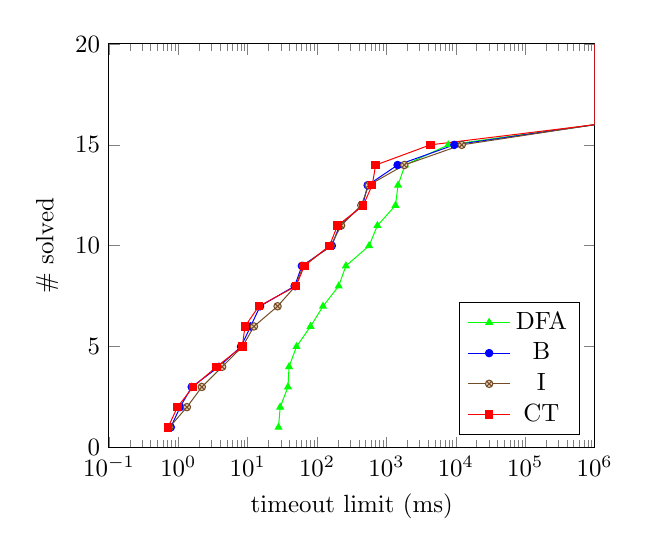
\begin{tikzpicture}[scale=0.9]
      \begin{axis}[
    xmode=log,
    ymin=0,ymax=20,
    xmin=0.1, xmax=1000000,
    every axis plot/.style={thin},
    xlabel={timeout limit (ms)},
    ylabel={\# solved},
    legend pos=south east
    % table/create on use/cumulative distribution/.style={
    %   create col/expr={\pgfmathaccuma + \thisrow{f(x)}}   
    % }
    ]
    \addplot 
    [mark=triangle*,
    mark size=1.5,
    mark options={solid},
    green] 
    coordinates {
    (27.813, 1)
(29.396, 2)
(38.090, 3)
(39.433, 4)
(50.529, 5)
(80.514, 6)
(121.723, 7)
(204.917, 8)
(260.270, 9)
(562.225, 10)
(740.384, 11)
(1350.760, 12)
(1468.227, 13)
(1850.035, 14)
(7773.486, 15)
(1000384.188, 16)
(1000415.992, 17)
(1001038.157, 18)
(1001164.640, 19)
(1002273.440, 20)
    };

    \addplot 
    [blue,
    mark=*,
    mark size=1.5,
    mark options={solid}]
    coordinates {
    (0.779, 1)
(1.060, 2)
(1.561, 3)
(3.839, 4)
(8.010, 5)
(11.021, 6)
(15.083, 7)
(47.529, 8)
(60.407, 9)
(163.209, 10)
(210.829, 11)
(454.146, 12)
(536.554, 13)
(1448.312, 14)
(9511.449, 15)
(1000105.287, 16)
(1000223.126, 17)
(1000233.215, 18)
(1000282.650, 19)
(1000507.490, 20)
    };

    \addplot [brown!60!black,
    mark options={fill=brown!40},
    mark=otimes*,
    mark size=1.5]
    coordinates {
    (0.745, 1)
(1.331, 2)
(2.184, 3)
(4.285, 4)
(8.411, 5)
(12.316, 6)
(26.960, 7)
(48.875, 8)
(63.114, 9)
(157.270, 10)
(222.204, 11)
(433.994, 12)
(555.190, 13)
(1808.071, 14)
(12163.199, 15)
(1000107.751, 16)
(1000130.129, 17)
(1000246.966, 18)
(1000291.968, 19)
(1000515.339, 20)
    };

    \addplot 
    [red,
    mark size=1.5,
    mark=square*]
    coordinates {
    (0.711, 1)
(0.972, 2)
(1.630, 3)
(3.558, 4)
(8.356, 5)
(9.137, 6)
(14.476, 7)
(49.775, 8)
(65.551, 9)
(150.785, 10)
(197.105, 11)
(462.423, 12)
(622.215, 13)
(699.950, 14)
(4293.162, 15)
(1000105.516, 16)
(1000116.994, 17)
(1000247.839, 18)
(1000308.963, 19)
(1000577.523, 20)
    };
    \legend{DFA,B,I,CT}
  \end{axis}

    \end{tikzpicture}
    \vfill
    \caption{\textbf{Langford 2}.}
    \vspace{\baselineskip}
  \end{minipage}\qquad
  \begin{minipage}[b][10cm][s]{0.45\textwidth}
    \centering
    \vfill
    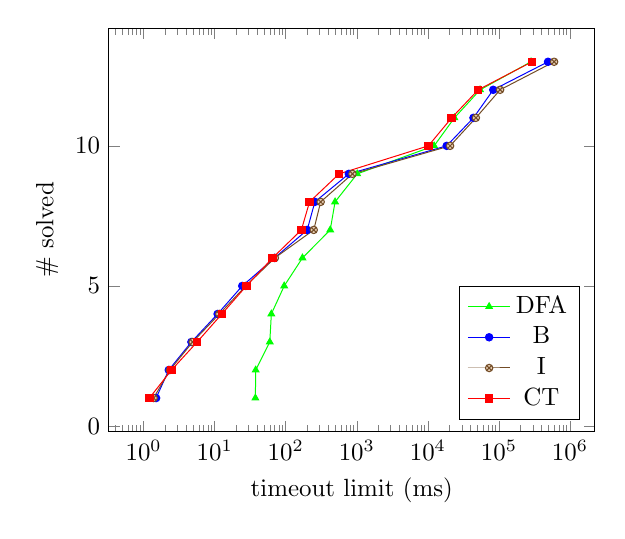
\begin{tikzpicture}[scale=0.9]
      \begin{axis}[
    xmode=log,
    every axis plot/.style={thin},
    xlabel={timeout limit (ms)},
    ylabel={\# solved},
    legend pos=south east
    % table/create on use/cumulative distribution/.style={
    %   create col/expr={\pgfmathaccuma + \thisrow{f(x)}}   
    % }
    ]
    \addplot 
    [mark=triangle*,
    mark size=1.5,
    mark options={solid},
    green] 
    coordinates {
    (37.414, 1)
(37.793, 2)
(59.679, 3)
(62.761, 4)
(95.181, 5)
(171.949, 6)
(422.923, 7)
(494.440, 8)
(1014.396, 9)
(12248.033, 10)
(23651.621, 11)
(54321.079, 12)
(283061.451, 13)
% (1002201.911, 14)
% (1002969.799, 15)
% (1004143.367, 16)
    };

    \addplot 
    [blue,
    mark=*,
    mark size=1.5,
    mark options={solid}]
    coordinates {
    (1.500, 1)
(2.262, 2)
(4.708, 3)
(11.004, 4)
(24.453, 5)
(69.784, 6)
(200.535, 7)
(257.119, 8)
(772.473, 9)
(18408.175, 10)
(43807.127, 11)
(83237.652, 12)
(490933.782, 13)
% (1000539.565, 14)
% (1000717.792, 15)
% (1000906.739, 16)
    };

    \addplot [brown!60!black,
    mark options={fill=brown!40},
    mark=otimes*,
    mark size=1.5]
    coordinates {
    (1.383, 1)
(2.345, 2)
(4.903, 3)
(11.647, 4)
(27.386, 5)
(70.258, 6)
(247.891, 7)
(310.355, 8)
(869.161, 9)
(20560.069, 10)
(47399.355, 11)
(103913.667, 12)
(597991.177, 13)
% (1000555.422, 14)
% (1000722.096, 15)
% (1000971.319, 16)
    };

    \addplot 
    [red,
    mark size=1.5,
    mark=square*]
    coordinates {
    (1.207, 1)
(2.472, 2)
(5.672, 3)
(12.628, 4)
(27.986, 5)
(65.314, 6)
(166.139, 7)
(216.350, 8)
(563.779, 9)
(10171.102, 10)
(21610.709, 11)
(51093.963, 12)
(291652.022, 13)
% (1000721.409, 14)
% (1000909.448, 15)
% (1001213.183, 16)
    };
    \legend{DFA,B,I,CT}
  \end{axis}

    \end{tikzpicture}
    \vfill
    \caption{\textbf{Langford 3}.}
    \vspace{\baselineskip}
  \end{minipage}\qquad
\end{figure}

\begin{figure}
  \begin{minipage}[b][10cm][s]{0.45\textwidth}
    \centering
    \vfill
    \begin{tikzpicture}[scale=0.9]
      \begin{axis}[
    xmode=log,
    every axis plot/.style={thin},
    xlabel={timeout limit (ms)},
    ylabel={\% solved},
    legend pos=south east,
    cycle list/Set1-6,
            % define fill color for the marker
            mark list fill={.!75!white},
            mark options={solid},
            cycle multiindex* list={
                Set1-6
                    \nextlist
                [3 of]linestyles
                    \nextlist
                very thick
                \nextlist
                mark=o,
                mark=*,
                mark=square,
                mark=triangle,
                mark=+
            },
    ]

    \addplot
    coordinates {
      (1410, 20)
      (2980, 40)
      (7950, 60)
      (22760, 80)
      (78820, 100)
      
    };
    \addplot
    coordinates {
      (650, 20)
      (1930, 40)
      (7810, 60)
      (29790, 80)
      (124670, 100)
      
    };
    \addplot
    coordinates {
      (740, 20)
      (2300, 40)
      (9460, 60)
      (36010, 80)
      (148310, 100)
      
    };
    \addplot
    coordinates {
      (580, 20)
      (1530, 40)
      (5640, 60)
      (20620, 80)
      (82360, 100)
      
    };
    

    \legend{ DFA, B, I, \textbf{CT} }
  \end{axis}

    \end{tikzpicture}
    \vfill
    \caption{\textbf{Langford 4}.}
    \vspace{\baselineskip}
  \end{minipage}\qquad
\end{figure}

\clearpage

\begin{figure}
  \begin{minipage}[b][10cm][s]{0.45\textwidth}
    \centering
    \vfill
    \begin{tikzpicture}[scale=0.9]
      \begin{axis}[
    xmode=log,
    every axis plot/.style={thin},
    xlabel={timeout limit (ms)},
    ylabel={\% solved},
    legend pos=south east,
    cycle list/Set1-6,
            % define fill color for the marker
            mark list fill={.!75!white},
            mark options={solid},
            cycle multiindex* list={
                Set1-6
                    \nextlist
                [3 of]linestyles
                    \nextlist
                very thick
                \nextlist
                mark=o,
                mark=*,
                mark=square,
                mark=triangle,
                mark=+
            },
    ]

    \addplot
    coordinates {
      (14650, 8)
      (14670, 15)
      (14940, 22)
      (15080, 29)
      (15100, 36)
      (15160, 43)
      (15400, 50)
      (15430, 58)
      (15440, 72)
      (15460, 79)
      (15560, 86)
      (15580, 93)
      (15640, 100)
      
    };
    \addplot
    coordinates {
      (1330, 8)
      (58080, 15)
      (401120, 22)
      (899860, 29)
      
    };
    \addplot
    coordinates {
      (2300, 8)
      (100420, 15)
      (538120, 22)
      
    };
    \addplot
    coordinates {
      (700, 8)
      (17280, 15)
      (142690, 22)
      (256150, 29)
      
    };
    

    \legend{ DFA, B, I, \textbf{CT} }
  \end{axis}

    \end{tikzpicture}
    \vfill
    \caption{\textbf{Mod Renault}.}
    \vspace{\baselineskip}
  \end{minipage}\qquad
  \begin{minipage}[b][10cm][s]{0.45\textwidth}
    \centering
    \vfill
    \begin{tikzpicture}[scale=0.9]
      \begin{axis}[
    xmode=log,
    every axis plot/.style={thin},
    xlabel={timeout limit (ms)},
    ylabel={\% solved},
    legend pos=south east,
    cycle list/Set1-6,
            % define fill color for the marker
            mark list fill={.!75!white},
            mark options={solid},
            cycle multiindex* list={
                Set1-6
                    \nextlist
                [3 of]linestyles
                    \nextlist
                very thick
                \nextlist
                mark=o,
                mark=*,
                mark=square,
                mark=triangle,
                mark=+
            },
    ]

    \addplot
    coordinates {
      (550, 7)
      (1420, 13)
      (2180, 19)
      (2460, 25)
      (4050, 32)
      (11860, 38)
      (37590, 44)
      (42030, 50)
      (51040, 57)
      (744510, 63)
      (828510, 69)
      (921350, 75)
      
    };
    \addplot
    coordinates {
      (730, 7)
      (2790, 13)
      (2950, 19)
      (9950, 25)
      (22390, 32)
      (55820, 38)
      (79890, 44)
      (247070, 50)
      
    };
    \addplot
    coordinates {
      (720, 7)
      (2880, 13)
      (4460, 19)
      (11570, 25)
      (21880, 32)
      (80590, 38)
      (84470, 44)
      (276470, 50)
      
    };
    \addplot
    coordinates {
      (140, 7)
      (210, 13)
      (680, 19)
      (1410, 25)
      (1760, 32)
      (2610, 38)
      (23590, 44)
      (29830, 50)
      (49050, 57)
      (474090, 63)
      (606460, 69)
      
    };
    

    \legend{ DFA, B, I, \textbf{CT} }
  \end{axis}

    \end{tikzpicture}
    \vfill
    \caption{\textbf{Pigeons Plus}.}
    \vspace{\baselineskip}
  \end{minipage}\qquad
\end{figure}

\begin{figure}
  \begin{minipage}[b][10cm][s]{0.45\textwidth}
    \centering
    \vfill
    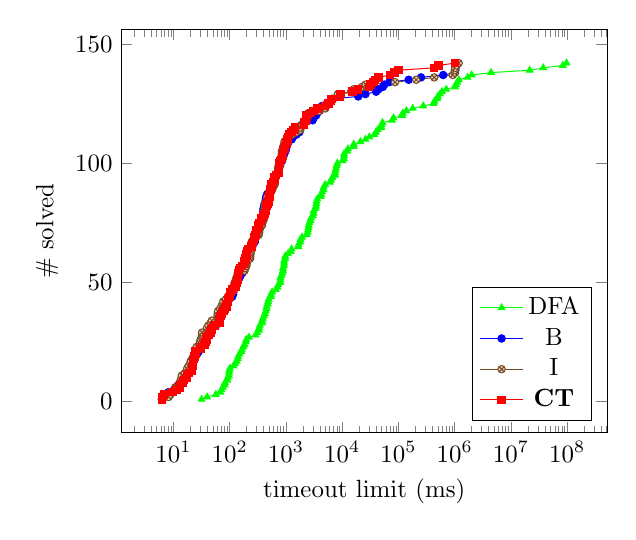
\begin{tikzpicture}[scale=0.9]
      \begin{axis}[
    xmode=log,
    every axis plot/.style={thin},
    xlabel={timeout limit (ms)},
    ylabel={\# solved},
    legend pos=south east
    % table/create on use/cumulative distribution/.style={
    %   create col/expr={\pgfmathaccuma + \thisrow{f(x)}}   
    % }
    ]
    \addplot 
    [mark=triangle*,
    mark size=1.5,
    mark options={solid},
    green] 
    coordinates {
    (31.696, 1)
(39.559, 2)
(56.508, 3)
(68.178, 4)
(70.931, 5)
(75.984, 6)
(81.689, 7)
(82.437, 8)
(90.551, 9)
(92.696, 10)
(96.318, 11)
(97.489, 12)
(98.251, 13)
(100.928, 14)
(116.739, 15)
(124.823, 16)
(132.967, 17)
(139.159, 18)
(141.636, 19)
(149.509, 20)
(161.219, 21)
(165.144, 22)
(176.745, 23)
(182.586, 24)
(193.826, 25)
(196.443, 26)
(220.596, 27)
(287.801, 28)
(307.637, 29)
(331.351, 30)
(335.110, 31)
(344.194, 32)
(377.529, 33)
(378.932, 34)
(389.655, 35)
(410.350, 36)
(423.248, 37)
(438.655, 38)
(450.859, 39)
(454.186, 40)
(475.260, 41)
(483.019, 42)
(493.122, 43)
(544.266, 44)
(544.377, 45)
(568.390, 46)
(658.959, 47)
(704.627, 48)
(733.115, 49)
(790.697, 50)
(796.819, 51)
(799.668, 52)
(839.106, 53)
(863.117, 54)
(884.469, 55)
(886.545, 56)
(921.009, 57)
(927.374, 58)
(928.500, 59)
(970.121, 60)
(970.451, 61)
(1084.311, 62)
(1214.035, 63)
(1256.732, 64)
(1667.050, 65)
(1679.067, 66)
(1790.603, 67)
(1813.082, 68)
(1923.256, 69)
(2334.693, 70)
(2424.581, 71)
(2460.778, 72)
(2524.488, 73)
(2535.289, 74)
(2608.483, 75)
(2727.527, 76)
(2790.777, 77)
(3010.831, 78)
(3089.396, 79)
(3100.186, 80)
(3342.097, 81)
(3421.319, 82)
(3476.286, 83)
(3498.766, 84)
(3603.983, 85)
(4152.208, 86)
(4252.733, 87)
(4414.005, 88)
(4619.485, 89)
(4703.303, 90)
(4995.143, 91)
(6104.482, 92)
(6327.657, 93)
(6680.221, 94)
(7451.205, 95)
(7524.283, 96)
(7577.742, 97)
(7815.366, 98)
(7963.806, 99)
(8190.616, 100)
(10239.338, 101)
(10646.387, 102)
(10743.772, 103)
(10816.354, 104)
(12183.647, 105)
(12608.953, 106)
(15986.466, 107)
(16016.047, 108)
(21085.457, 109)
(25840.612, 110)
(30330.074, 111)
(37303.992, 112)
(39784.632, 113)
(42867.757, 114)
(49654.939, 115)
(49896.816, 116)
(51937.811, 117)
(76626.715, 118)
(81762.693, 119)
(116690.715, 120)
(118979.114, 121)
(138352.575, 122)
(179596.690, 123)
(275896.959, 124)
(422494.853, 125)
(435710.733, 126)
(490650.459, 127)
(500154.998, 128)
(546044.177, 129)
(592457.334, 130)
(707795.890, 131)
(1014847.682, 132)
(1051973.108, 133)
(1109712.990, 134)
(1188811.633, 135)
(1691073.549, 136)
(1998815.209, 137)
(4412151.304, 138)
(21464315.090, 139)
(37446981.305, 140)
(83163795.720, 141)
(97236200.525, 142)
    };

    \addplot 
    [blue,
    mark=*,
    mark size=1.5,
    mark options={solid}]
    coordinates {
    (6.266, 1)
(6.620, 2)
(7.191, 3)
(8.174, 4)
(10.291, 5)
(11.099, 6)
(12.126, 7)
(13.714, 8)
(14.201, 9)
(17.122, 10)
(17.173, 11)
(18.736, 12)
(19.358, 13)
(19.989, 14)
(20.187, 15)
(20.291, 16)
(20.437, 17)
(21.788, 18)
(22.787, 19)
(26.326, 20)
(28.086, 21)
(28.501, 22)
(30.269, 23)
(30.327, 24)
(31.429, 25)
(32.957, 26)
(35.312, 27)
(37.683, 28)
(42.027, 29)
(44.010, 30)
(45.270, 31)
(57.413, 32)
(58.136, 33)
(60.287, 34)
(63.612, 35)
(64.377, 36)
(70.203, 37)
(71.636, 38)
(74.510, 39)
(81.417, 40)
(81.885, 41)
(86.850, 42)
(98.379, 43)
(110.554, 44)
(114.955, 45)
(116.342, 46)
(116.797, 47)
(117.697, 48)
(127.569, 49)
(128.638, 50)
(132.319, 51)
(149.619, 52)
(156.554, 53)
(167.748, 54)
(171.866, 55)
(177.579, 56)
(186.974, 57)
(188.731, 58)
(197.746, 59)
(206.427, 60)
(212.854, 61)
(223.093, 62)
(234.349, 63)
(237.887, 64)
(249.281, 65)
(261.335, 66)
(279.625, 67)
(282.633, 68)
(287.627, 69)
(297.860, 70)
(315.101, 71)
(322.909, 72)
(331.748, 73)
(351.193, 74)
(352.948, 75)
(363.872, 76)
(366.739, 77)
(390.571, 78)
(395.284, 79)
(397.359, 80)
(399.002, 81)
(410.756, 82)
(418.082, 83)
(436.759, 84)
(439.198, 85)
(447.297, 86)
(462.840, 87)
(504.442, 88)
(543.477, 89)
(559.175, 90)
(566.240, 91)
(601.149, 92)
(619.715, 93)
(652.612, 94)
(657.839, 95)
(715.983, 96)
(731.157, 97)
(752.783, 98)
(784.906, 99)
(794.121, 100)
(856.340, 101)
(862.438, 102)
(901.933, 103)
(927.762, 104)
(979.127, 105)
(1000.759, 106)
(1023.428, 107)
(1067.513, 108)
(1074.968, 109)
(1265.279, 110)
(1331.799, 111)
(1538.059, 112)
(1731.374, 113)
(1737.023, 114)
(1790.519, 115)
(1895.419, 116)
(2041.525, 117)
(2975.267, 118)
(3105.441, 119)
(3430.058, 120)
(3574.657, 121)
(3985.434, 122)
(4137.262, 123)
(4364.834, 124)
(5314.336, 125)
(6189.835, 126)
(6463.719, 127)
(19294.688, 128)
(25874.502, 129)
(40075.340, 130)
(44076.314, 131)
(52831.470, 132)
(56117.125, 133)
(69049.283, 134)
(151946.681, 135)
(251788.612, 136)
(624723.233, 137)
(1006224.760, 138)
(1024927.746, 139)
(1025126.900, 140)
(1051096.785, 141)
(1054709.554, 142)
    };

    \addplot [brown!60!black,
    mark options={fill=brown!40},
    mark=otimes*,
    mark size=1.5]
    coordinates {
    (6.225, 1)
(8.252, 2)
(8.866, 3)
(8.903, 4)
(10.276, 5)
(10.793, 6)
(12.246, 7)
(12.967, 8)
(13.482, 9)
(13.873, 10)
(14.125, 11)
(15.975, 12)
(17.388, 13)
(17.590, 14)
(18.641, 15)
(20.043, 16)
(20.476, 17)
(21.613, 18)
(23.615, 19)
(24.164, 20)
(24.372, 21)
(24.882, 22)
(26.053, 23)
(29.400, 24)
(29.513, 25)
(30.549, 26)
(31.898, 27)
(32.205, 28)
(32.366, 29)
(39.353, 30)
(39.524, 31)
(42.127, 32)
(45.853, 33)
(48.185, 34)
(60.297, 35)
(60.940, 36)
(61.286, 37)
(61.970, 38)
(67.684, 39)
(71.354, 40)
(74.374, 41)
(76.755, 42)
(86.492, 43)
(92.532, 44)
(102.074, 45)
(107.118, 46)
(110.458, 47)
(119.452, 48)
(120.692, 49)
(122.537, 50)
(130.211, 51)
(131.757, 52)
(139.069, 53)
(139.341, 54)
(184.184, 55)
(187.471, 56)
(198.576, 57)
(201.040, 58)
(207.945, 59)
(229.958, 60)
(232.188, 61)
(233.976, 62)
(239.163, 63)
(240.688, 64)
(241.932, 65)
(243.311, 66)
(245.547, 67)
(265.954, 68)
(292.029, 69)
(328.546, 70)
(334.072, 71)
(336.358, 72)
(350.752, 73)
(375.324, 74)
(379.234, 75)
(396.967, 76)
(401.683, 77)
(401.895, 78)
(405.570, 79)
(411.227, 80)
(417.570, 81)
(419.966, 82)
(421.977, 83)
(456.664, 84)
(458.121, 85)
(467.458, 86)
(514.809, 87)
(537.183, 88)
(573.529, 89)
(585.083, 90)
(628.983, 91)
(629.151, 92)
(638.579, 93)
(655.494, 94)
(683.596, 95)
(719.854, 96)
(720.103, 97)
(726.177, 98)
(743.018, 99)
(776.859, 100)
(788.068, 101)
(801.667, 102)
(840.869, 103)
(844.819, 104)
(845.660, 105)
(882.665, 106)
(896.694, 107)
(936.968, 108)
(941.257, 109)
(1025.243, 110)
(1127.272, 111)
(1290.616, 112)
(1527.467, 113)
(1798.817, 114)
(1803.072, 115)
(1966.245, 116)
(2089.371, 117)
(2225.216, 118)
(2378.815, 119)
(2497.087, 120)
(2503.823, 121)
(3943.794, 122)
(5004.718, 123)
(5143.946, 124)
(5663.752, 125)
(6369.410, 126)
(6913.053, 127)
(8260.886, 128)
(8382.946, 129)
(14367.240, 130)
(16013.595, 131)
(22433.224, 132)
(26100.534, 133)
(86936.175, 134)
(206857.036, 135)
(432302.057, 136)
(923791.300, 137)
(1001275.049, 138)
(1005552.392, 139)
(1024252.398, 140)
(1082346.127, 141)
(1174868.682, 142)
    };

    \addplot 
    [red,
    mark size=1.5,
    mark=square*]
    coordinates {
    (6.328, 1)
(6.344, 2)
(6.785, 3)
(9.703, 4)
(11.389, 5)
(12.785, 6)
(13.199, 7)
(14.710, 8)
(15.330, 9)
(17.053, 10)
(17.466, 11)
(18.730, 12)
(21.191, 13)
(21.458, 14)
(22.190, 15)
(22.321, 16)
(22.429, 17)
(23.230, 18)
(23.566, 19)
(24.810, 20)
(24.843, 21)
(30.529, 22)
(31.162, 23)
(35.615, 24)
(37.410, 25)
(38.475, 26)
(38.831, 27)
(43.209, 28)
(45.793, 29)
(47.775, 30)
(48.066, 31)
(53.755, 32)
(65.633, 33)
(66.267, 34)
(66.798, 35)
(69.198, 36)
(73.621, 37)
(77.636, 38)
(83.309, 39)
(87.127, 40)
(87.800, 41)
(92.901, 42)
(93.082, 43)
(98.471, 44)
(101.548, 45)
(102.853, 46)
(112.950, 47)
(126.755, 48)
(126.916, 49)
(133.777, 50)
(136.483, 51)
(139.301, 52)
(141.708, 53)
(142.901, 54)
(147.720, 55)
(151.267, 56)
(167.047, 57)
(180.053, 58)
(185.002, 59)
(192.458, 60)
(199.346, 61)
(200.444, 62)
(205.194, 63)
(211.032, 64)
(245.046, 65)
(247.635, 66)
(258.985, 67)
(273.140, 68)
(274.226, 69)
(289.992, 70)
(293.258, 71)
(296.666, 72)
(320.259, 73)
(325.794, 74)
(331.950, 75)
(359.459, 76)
(369.740, 77)
(401.942, 78)
(428.598, 79)
(439.186, 80)
(443.919, 81)
(451.155, 82)
(465.721, 83)
(486.636, 84)
(496.533, 85)
(507.498, 86)
(509.344, 87)
(518.391, 88)
(534.298, 89)
(549.969, 90)
(554.731, 91)
(594.595, 92)
(623.445, 93)
(624.194, 94)
(658.888, 95)
(748.721, 96)
(754.742, 97)
(754.776, 98)
(757.089, 99)
(766.244, 100)
(789.618, 101)
(856.352, 102)
(878.697, 103)
(882.688, 104)
(885.633, 105)
(948.909, 106)
(961.811, 107)
(1025.381, 108)
(1027.979, 109)
(1068.881, 110)
(1096.069, 111)
(1141.179, 112)
(1263.836, 113)
(1363.480, 114)
(1444.963, 115)
(2086.545, 116)
(2104.289, 117)
(2266.072, 118)
(2315.715, 119)
(2337.155, 120)
(2809.498, 121)
(3062.328, 122)
(3613.655, 123)
(4962.131, 124)
(5757.448, 125)
(6278.281, 126)
(6458.606, 127)
(9074.926, 128)
(9388.538, 129)
(15237.846, 130)
(19012.640, 131)
(29844.102, 132)
(32057.652, 133)
(36009.393, 134)
(38516.958, 135)
(44360.448, 136)
(70712.723, 137)
(84815.013, 138)
(99208.278, 139)
(426595.818, 140)
(513749.533, 141)
(1012388.065, 142)
    };
    \legend{DFA,B,I,\textbf{CT}}
  \end{axis}

    \end{tikzpicture}
    \vfill
    \caption{\textbf{Nonograms}.}
    \vspace{\baselineskip}
  \end{minipage}\qquad
  \begin{minipage}[b][10cm][s]{0.45\textwidth}
    \centering
    \vfill
    \begin{tikzpicture}[scale=0.9]
      \begin{axis}[
    xmode=log,
    every axis plot/.style={thin},
    xlabel={timeout limit (ms)},
    ylabel={\% solved},
    legend pos=south east,
    cycle list/Set1-6,
            % define fill color for the marker
            mark list fill={.!75!white},
            mark options={solid},
            cycle multiindex* list={
                Set1-6
                    \nextlist
                [3 of]linestyles
                    \nextlist
                very thick
                \nextlist
                mark=o,
                mark=*,
                mark=square,
                mark=triangle,
                mark=+
            },
    ]

    \addplot
    coordinates {
      (674950, 6)
      
    };
    \addplot
    coordinates {
      (1005060, 6)
      
    };
    \addplot
    coordinates {
      (1005070, 6)
      
    };
    \addplot
    coordinates {
      (31500, 6)
      (63030, 12)
      (409250, 18)
      (694360, 24)
      (805460, 30)
      (942180, 36)
      (995270, 42)
      
    };
    

    \legend{ DFA, B, I, \textbf{CT} }
  \end{axis}

    \end{tikzpicture}
    \vfill
    \caption{\textbf{MDD 05}.}
    \vspace{\baselineskip}
  \end{minipage}\qquad
\end{figure}

\clearpage

\begin{figure}
  \begin{minipage}[b][10cm][s]{.45\textwidth}
     \centering
    \vfill
    \begin{tikzpicture}[scale=0.9]
      \begin{axis}[
    xmode=log,
    every axis plot/.style={thin},
    xlabel={timeout limit (ms)},
    ylabel={\% solved},
    legend style={at={(0.5,-0.30)},
      anchor=north,legend columns=-1},
    % legend pos=south east,
    cycle list/Set1-6,
            % define fill color for the marker
            mark list fill={.!75!white},
            mark options={solid,scale=0.9},
            cycle multiindex* list={
                Set1-6
                    \nextlist
                [3 of]linestyles
                    \nextlist
                very thick
                \nextlist
                mark=o,
                mark=*,
                mark=square,
                mark=triangle,
                mark=+
            },
    ]

    \addplot
    coordinates {
      (5430, 10)
      (14920, 20)
      (15140, 30)
      (16070, 40)
      (39070, 50)
      (55650, 60)
      (68040, 70)
      (98270, 80)
      (136850, 90)
      (547470, 100)
      
    };
    \addplot
    coordinates {
      (2210, 10)
      (5690, 20)
      (6980, 30)
      (8620, 40)
      (21410, 50)
      (25040, 60)
      (42340, 70)
      (57090, 80)
      (61660, 90)
      (253910, 100)
      
    };
    \addplot
    coordinates {
      (3120, 10)
      (9260, 20)
      (10590, 30)
      (12520, 40)
      (31430, 50)
      (37860, 60)
      (61840, 70)
      (82360, 80)
      (95870, 90)
      (382470, 100)
      
    };
    \addplot
    coordinates {
      (580, 10)
      (1260, 20)
      (1420, 30)
      (1590, 40)
      (3560, 50)
      (4040, 60)
      (6340, 70)
      (8660, 80)
      (9980, 90)
      (43230, 100)
      
    };
    

    \legend{ DFA, B, I, \textbf{CT} }
  \end{axis}

    \end{tikzpicture}    
    \vfill
    \caption{\textbf{Rands JC2500.}}
    \vspace{\baselineskip}
  \end{minipage}\qquad
  \begin{minipage}[b][10cm][s]{.45\textwidth}
    \centering
    \vfill
    \begin{tikzpicture}[scale=0.9]
      \begin{axis}[
    xmode=log,
    every axis plot/.style={thin},
    xlabel={timeout limit (ms)},
    ylabel={\% solved},
    legend pos=south east,
    cycle list/Set1-6,
            % define fill color for the marker
            mark list fill={.!75!white},
            mark options={solid},
            cycle multiindex* list={
                Set1-6
                    \nextlist
                [3 of]linestyles
                    \nextlist
                very thick
                \nextlist
                mark=o,
                mark=*,
                mark=square,
                mark=triangle,
                mark=+
            },
    ]

    \addplot
    coordinates {
      (34430, 20)
      (60980, 40)
      (97460, 60)
      (376360, 80)
      (382430, 100)
      
    };
    \addplot
    coordinates {
      (20900, 20)
      (29740, 40)
      (45540, 60)
      (225660, 80)
      (273020, 100)
      
    };
    \addplot
    coordinates {
      (27430, 20)
      (43410, 40)
      (68070, 60)
      (313020, 80)
      (361180, 100)
      
    };
    \addplot
    coordinates {
      (3110, 20)
      (3570, 40)
      (6150, 60)
      (24650, 80)
      (27780, 100)
      
    };
    

    \legend{ DFA, B, I, \textbf{CT} }
  \end{axis}

    \end{tikzpicture}
    \vfill
    \caption{\textbf{Rands JC5000.}}
    \vspace{\baselineskip}
  \end{minipage}\qquad
\end{figure}

\begin{figure}
    \begin{minipage}[b][10cm][s]{.45\textwidth}
    \centering
    \vfill
    \begin{tikzpicture}[scale=0.9]
      \begin{axis}[
    xmode=log,
    every axis plot/.style={thin},
    xlabel={timeout limit (ms)},
    ylabel={\% solved},
    legend pos=south east,
    cycle list/Set1-6,
            % define fill color for the marker
            mark list fill={.!75!white},
            mark options={solid},
            cycle multiindex* list={
                Set1-6
                    \nextlist
                [3 of]linestyles
                    \nextlist
                very thick
                \nextlist
                mark=o,
                mark=*,
                mark=square,
                mark=triangle,
                mark=+
            },
    ]

    \addplot
    coordinates {
      (141410, 10)
      (147100, 20)
      (188630, 30)
      (439630, 40)
      
    };
    \addplot
    coordinates {
      (81770, 10)
      (105640, 20)
      (117810, 30)
      (259930, 40)
      (777770, 50)
      (901390, 60)
      
    };
    \addplot
    coordinates {
      (113550, 10)
      (137140, 20)
      (156920, 30)
      (342630, 40)
      
    };
    \addplot
    coordinates {
      (7730, 10)
      (11520, 20)
      (12470, 30)
      (26010, 40)
      (72590, 50)
      (80830, 60)
      (133710, 70)
      (275860, 80)
      (623230, 90)
      
    };
    

    \legend{ DFA, B, I, \textbf{CT} }
  \end{axis}

    \end{tikzpicture}
    \vfill
    \caption{\textbf{Rands JC7500}.}
    \vspace{\baselineskip}
  \end{minipage}\qquad
  \begin{minipage}[b][10cm][s]{.45\textwidth}
    \centering
    \vfill
    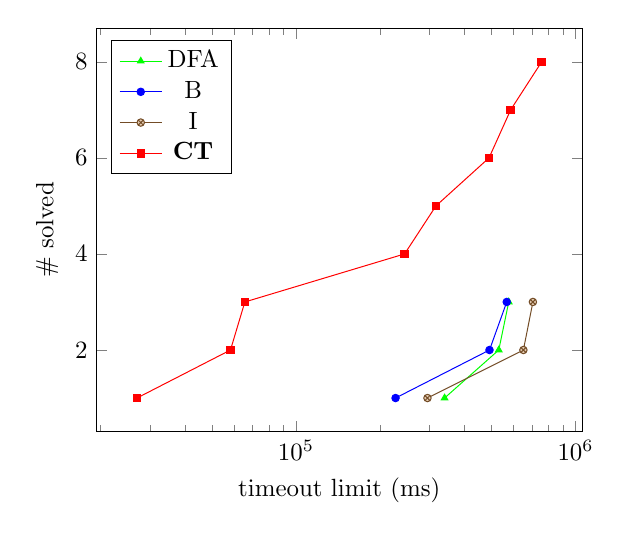
\begin{tikzpicture}[scale=0.9]
      \begin{axis}[
    xmode=log,
    every axis plot/.style={thin},
    xlabel={timeout limit (ms)},
    ylabel={\# solved},
    legend pos=north west
    % table/create on use/cumulative distribution/.style={
    %   create col/expr={\pgfmathaccuma + \thisrow{f(x)}}   
    % }
    ]
    \addplot 
    [mark=triangle*,
    mark size=1.5,
    mark options={solid},
    green] 
    coordinates {
    (339960.449, 1)
(531357.500, 2)
(576758.002, 3)
% (1006830.253, 4)
% (1006953.686, 5)
% (1006987.278, 6)
% (1007012.182, 7)
% (1007040.479, 8)
% (1007166.422, 9)
% (1007385.382, 10)
    };

    \addplot 
    [blue,
    mark=*,
    mark size=1.5,
    mark options={solid}]
    coordinates {
    (227052.199, 1)
(492242.811, 2)
(567372.313, 3)
% (1000877.234, 4)
% (1000889.042, 5)
% (1000892.874, 6)
% (1000895.207, 7)
% (1000911.856, 8)
% (1000913.878, 9)
% (1000928.789, 10)
    };

    \addplot [brown!60!black,
    mark options={fill=brown!40},
    mark=otimes*,
    mark size=1.5]
    coordinates {
    (295287.152, 1)
(650810.991, 2)
(703794.608, 3)
% (1000887.426, 4)
% (1000895.815, 5)
% (1000897.600, 6)
% (1000901.551, 7)
% (1000905.923, 8)
% (1000907.888, 9)
% (1000913.436, 10)
    };

    \addplot 
    [red,
    mark size=1.5,
    mark=square*]
    coordinates {
    (26984.703, 1)
(58304.179, 2)
(65624.179, 3)
(244616.117, 4)
(316746.918, 5)
(490346.243, 6)
(586068.768, 7)
(756641.057, 8)
%(1001171.576, 9)
%(1001192.839, 10)
    };
    \legend{DFA,B,I,\textbf{CT}}
  \end{axis}

    \end{tikzpicture}
    \vfill
    \caption{\textbf{Rands JC10000}.}
    \vspace{\baselineskip}
  \end{minipage}\qquad

\end{figure}

\clearpage

\begin{figure}
  \begin{minipage}[b][10cm][s]{0.45\textwidth}
    \centering
    \vfill
    \begin{tikzpicture}[scale=0.9]
      \begin{axis}[
    xmode=log,
    every axis plot/.style={thin},
    xlabel={timeout limit (ms)},
    ylabel={\% solved},
    legend pos=south east,
    cycle list/Set1-6,
            % define fill color for the marker
            mark list fill={.!75!white},
            mark options={solid},
            cycle multiindex* list={
                Set1-6
                    \nextlist
                [3 of]linestyles
                    \nextlist
                very thick
                \nextlist
                mark=o,
                mark=*,
                mark=square,
                mark=triangle,
                mark=+
            },
    ]

    \addplot
    coordinates {
      (1110, 7)
      (1760, 14)
      (2010, 20)
      (2590, 27)
      (3550, 34)
      (5220, 40)
      (5280, 47)
      (5520, 54)
      (6530, 60)
      (6800, 67)
      (7760, 74)
      (8950, 80)
      (9580, 87)
      (10970, 94)
      (18580, 100)
      
    };
    \addplot
    coordinates {
      (100, 7)
      (130, 14)
      (190, 20)
      (220, 27)
      (350, 34)
      (1150, 40)
      (1210, 47)
      (2080, 54)
      (3850, 60)
      (3960, 67)
      (4020, 74)
      (5380, 80)
      (7810, 87)
      (12090, 94)
      (31300, 100)
      
    };
    \addplot
    coordinates {
      (110, 7)
      (140, 14)
      (220, 20)
      (240, 27)
      (410, 34)
      (1550, 40)
      (1730, 47)
      (2910, 54)
      (5410, 60)
      (5510, 67)
      (5980, 74)
      (7980, 80)
      (11090, 87)
      (16680, 94)
      (46730, 100)
      
    };
    \addplot
    coordinates {
      (110, 7)
      (140, 14)
      (170, 20)
      (190, 27)
      (270, 34)
      (610, 47)
      (1030, 54)
      (1700, 67)
      (1750, 74)
      (2080, 80)
      (3460, 87)
      (4610, 94)
      (11740, 100)
      
    };
    

    \legend{ DFA, B, I, \textbf{CT} }
  \end{axis}

    \end{tikzpicture}
    \vfill
    \caption{\textbf{TSP 20}.}
    \vspace{\baselineskip}
  \end{minipage}\qquad
  \begin{minipage}[b][10cm][s]{0.45\textwidth}
    \centering
    \vfill
    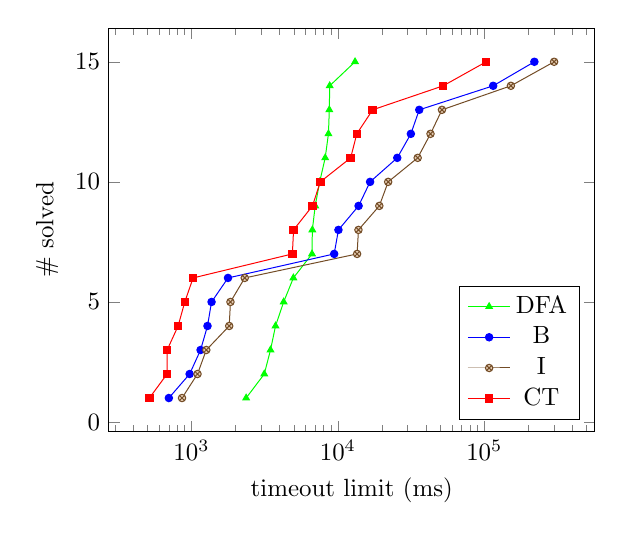
\begin{tikzpicture}[scale=0.9]
      \begin{axis}[
    xmode=log,
    every axis plot/.style={thin},
    xlabel={timeout limit (ms)},
    ylabel={\# solved},
    legend pos=south east
    % table/create on use/cumulative distribution/.style={
    %   create col/expr={\pgfmathaccuma + \thisrow{f(x)}}   
    % }
    ]
    \addplot 
    [mark=triangle*,
    mark size=1.5,
    mark options={solid},
    green] 
    coordinates {
    (2363.505, 1)
(3143.552, 2)
(3466.877, 3)
(3752.121, 4)
(4263.437, 5)
(4967.203, 6)
(6659.753, 7)
(6693.385, 8)
(7000.752, 9)
(7512.368, 10)
(8191.457, 11)
(8621.325, 12)
(8742.062, 13)
(8792.607, 14)
(13100.321, 15)
    };

    \addplot 
    [blue,
    mark=*,
    mark size=1.5,
    mark options={solid}]
    coordinates {
    (701.119, 1)
(971.999, 2)
(1154.302, 3)
(1287.150, 4)
(1372.015, 5)
(1777.244, 6)
(9433.727, 7)
(10090.615, 8)
(13850.887, 9)
(16597.978, 10)
(25440.103, 11)
(31511.070, 12)
(35953.450, 13)
(114961.468, 14)
(219755.844, 15)
    };

    \addplot [brown!60!black,
    mark options={fill=brown!40},
    mark=otimes*,
    mark size=1.5]
    coordinates {
    (862.363, 1)
(1099.916, 2)
(1262.976, 3)
(1811.278, 4)
(1846.992, 5)
(2311.755, 6)
(13529.833, 7)
(13821.151, 8)
(19187.557, 9)
(22056.404, 10)
(35072.499, 11)
(42907.328, 12)
(51387.532, 13)
(151853.872, 14)
(299791.408, 15)
    };

    \addplot 
    [red,
    mark size=1.5,
    mark=square*]
    coordinates {
    (516.336, 1)
(681.894, 2)
(682.555, 3)
(810.895, 4)
(900.771, 5)
(1026.305, 6)
(4888.873, 7)
(4982.325, 8)
(6709.139, 9)
(7587.633, 10)
(12227.579, 11)
(13464.500, 12)
(17279.083, 13)
(52420.089, 14)
(102983.567, 15)
    };
    \legend{DFA,B,I,CT}
  \end{axis}

    \end{tikzpicture}
    \vfill
    \caption{\textbf{TSP 25}.}
    \vspace{\baselineskip}
  \end{minipage}\qquad
\end{figure}


\begin{figure}
  \begin{minipage}[b][10cm][s]{0.45\textwidth}
    \centering
    \vfill
    \begin{tikzpicture}[scale=0.9]
      \begin{axis}[
    xmode=log,
    every axis plot/.style={thin},
    xlabel={timeout limit (ms)},
    ylabel={\% solved},
    legend pos=south east,
    cycle list/Set1-6,
            % define fill color for the marker
            mark list fill={.!75!white},
            mark options={solid},
            cycle multiindex* list={
                Set1-6
                    \nextlist
                [3 of]linestyles
                    \nextlist
                very thick
                \nextlist
                mark=o,
                mark=*,
                mark=square,
                mark=triangle,
                mark=+
            },
    ]

    \addplot
    coordinates {
      (9270, 7)
      (9500, 14)
      (9650, 20)
      (10200, 27)
      (11200, 34)
      (12670, 40)
      (13740, 47)
      (13820, 54)
      (14320, 60)
      (14650, 67)
      (16050, 74)
      (16730, 80)
      (19980, 87)
      (20820, 94)
      (32170, 100)
      
    };
    \addplot
    coordinates {
      (1230, 7)
      (1240, 14)
      (1600, 20)
      (1620, 27)
      (2220, 34)
      (6140, 40)
      (7350, 47)
      (11490, 54)
      (20670, 60)
      (22400, 67)
      (23060, 74)
      (39870, 80)
      (42730, 87)
      (72970, 94)
      (189860, 100)
      
    };
    \addplot
    coordinates {
      (1180, 7)
      (1290, 14)
      (2150, 20)
      (2250, 27)
      (3660, 34)
      (12210, 40)
      (15470, 47)
      (23680, 54)
      (44370, 60)
      (50400, 67)
      (53220, 74)
      (88220, 80)
      (93840, 87)
      (162560, 94)
      (437270, 100)
      
    };
    \addplot
    coordinates {
      (1260, 7)
      (1310, 14)
      (1370, 20)
      (1500, 27)
      (1520, 34)
      (1910, 40)
      (1950, 47)
      (3140, 54)
      (4410, 60)
      (4970, 67)
      (5830, 74)
      (7210, 80)
      (9790, 87)
      (12870, 94)
      (34120, 100)
      
    };
    

    \legend{ DFA, B, I, \textbf{CT} }
  \end{axis}

    \end{tikzpicture}
    \vfill
    \caption{\textbf{TSP Quat 20}.}
    \vspace{\baselineskip}
  \end{minipage}\qquad
\end{figure}

\clearpage


